\documentclass[12pt,openany,a4paper]{book}
\usepackage{graphics}	% if you want encapsulated PS figures.
\usepackage{spverbatim}
\usepackage{alltt}
\usepackage{graphics}
% If you use a macro file called macros.tex :
% \input{macros}
% Note: The present document has its macros built in.

% Number subsections but not subsubsections:
\setcounter{secnumdepth}{2}
% Show subsections but not subsubsections in table of contents:
\setcounter{tocdepth}{2}

\pagestyle{headings}		% Chapter on left page, Section on right.
\raggedbottom

\setlength{\topmargin}		{-5mm}  %  25-5 = 20mm
\setlength{\oddsidemargin}	{10mm}  % rhs page inner margin = 25+10mm
\setlength{\evensidemargin}	{0mm}   % lhs page outer margin = 25mm
\setlength{\textwidth}		{150mm} % 35 + 150 + 25 = 210mm
\setlength{\textheight}		{240mm} % 

\renewcommand{\baselinestretch}{1.2}	% Looks like 1.5 spacing.

% Stop figure/tables smaller than 3/4 page from appearing alone on a page:
\renewcommand{\textfraction}{0.25}
\renewcommand{\topfraction}{0.75}
\renewcommand{\bottomfraction}{0.75}
\renewcommand{\floatpagefraction}{0.75}

% THEOREM-LIKE ENVIRONMENTS:
\newtheorem{defn}	{Definition}	% cf. \dfn for cross-referencing
\newtheorem{theorem}	{Theorem}	% cf. \thrm for cross-referencing
\newtheorem{lemma}	{Lemma}		% cf. \lem for cross-referencing

% AIDS TO CROSS-REFERENCING (All take a label as argument):
\newcommand{\eref}[1] {(\ref{#1})}		% (...)
\newcommand{\eq}[1]   {Eq.\,(\ref{#1})}		% Eq.~(...)
\newcommand{\eqs}[2]  {Eqs.~(\ref{#1}) and~(\ref{#2})}
\newcommand{\dfn}[1]  {Definition~\ref{#1}}	% Definition~...
\newcommand{\thrm}[1] {Theorem~\ref{#1}}	% Theorem~...
\newcommand{\lem}[1]  {Lemma~\ref{#1}}		% Lemma~...
\newcommand{\fig}[1]  {Fig.\,\ref{#1}}		% Fig.~...
\newcommand{\tab}[1]  {Table~\ref{#1}}		% Table~...
\newcommand{\chap}[1] {Chapter~\ref{#1}}	% Chapter~...
\newcommand{\secn}[1] {Section~\ref{#1}}	% Section~...
\newcommand{\ssec}[1] {Subsection~\ref{#1}}	% Subsection~...

% AIDS TO FORMATTING:
\newcommand{\teq}[1]	{\mbox{$#1$}}	% in-Text EQuation (unbreakable)
\newcommand{\qed}	{\hspace*{\fill}$\bullet$}	% end of proof

% MATHEMATICAL TEMPLATES:
% Text or math mode:
\newcommand{\half}	{\ensuremath{\frac{1}{2}}}	% one-half
\newcommand{\halftxt}	{\mbox{$\frac{1}{2}$}}	  	% one-half, small
% Math mode only:
% N.B. Parentheses are ROUND; brackets are SQUARE!
\newcommand{\oneon}[1]	{\frac{1}{#1}}		  % reciprocal
\newcommand{\pow}[2]	{\left({#1}\right)^{#2}}  % Parenthesized pOWer
\newcommand{\bow}[2]	{\left[{#1}\right]^{#2}}  % Bracketed pOWer
\newcommand{\evalat}[2]	{\left.{#1}\right|_{#2}}  % EVALuated AT with bar
\newcommand{\bevalat}[2]{\left[{#1}\right]_{#2}}  % Bracketed EVALuated AT
% Total derivatives:
\newcommand{\sdd}[2]	{\frac{d{#1}}{d{#2}}}		    % Short
\newcommand{\sqdd}[2]	{\frac{d^2{#1}}{d{#2}^2}}	    % 2nd ("SQuared")
\newcommand{\ldd}[2]	{\frac{d}{d{#1}}\left({#2}\right)}  % Long paren'ed
\newcommand{\bdd}[2]	{\frac{d}{d{#2}}\left[{#2}\right]}  % long Bracketed
% Partial derivatives (same sequence as for total derivatives):
\newcommand{\sdada}[2]	{\frac{\partial {#1}}{\partial {#2}}}
\newcommand{\sqdada}[2]	{\frac{\partial ^{2}{#1}}{\partial {#2}^{2}}}
\newcommand{\ldada}[2]	{\frac{\partial}{\partial {#1}}\left({#2}\right)}
\newcommand{\bdada}[2]	{\frac{\partial}{\partial {#1}}\left[{#2}\right]}
\newcommand{\da}	{\partial}

% ORDINAL NUMBERS:
\newcommand{\ith}	{\ensuremath{i^{\rm th}}}
\newcommand{\jth}	{\ensuremath{j^{\rm th}}}
\newcommand{\kth}	{\ensuremath{k^{\rm th}}}
\newcommand{\lth}	{\ensuremath{l^{\rm th}}}
\newcommand{\mth}	{\ensuremath{m^{\rm th}}}
\newcommand{\nth}	{\ensuremath{n^{\rm th}}}

% SINUSOIDAL TIME AND SPACE-DEPENDENCY FACTORS:
\newcommand{\ejot}	{\ensuremath{e^{j\omega t}}}
\newcommand{\emjot}	{\ensuremath{e^{-j\omega t}}}

% UNITS (TEXT OR MATH MODE, WITH LEADING PADDING SPACE IF APPLICABLE):
% NB: These have not been tested since being modified for LaTeX2e.
\newcommand{\pack}	{\hspace{-0.08em}}
\newcommand{\Pack}	{\hspace{-0.12em}}
\newcommand{\mA}	{\ensuremath{\rm\,m\pack A}}
\newcommand{\dB}	{\ensuremath{\rm\,d\pack B}}
\newcommand{\dBm}	{\ensuremath{\rm\,d\pack B\pack m}}
\newcommand{\dBW}	{\ensuremath{\rm\,d\pack B\Pack W}}
\newcommand{\uF}	{\ensuremath{\rm\,\mu\pack F}}
\newcommand{\pF}	{\ensuremath{\rm\,p\pack F}}
\newcommand{\nF}	{\ensuremath{\rm\,n\pack F}}
\newcommand{\uH}	{\ensuremath{\rm\,\mu\pack H}}
\newcommand{\mH}	{\ensuremath{\rm\,m\pack H}}
\newcommand{\Hz}	{\ensuremath{\rm\,H\pack z}}
\newcommand{\kHz}	{\ensuremath{\rm\,k\pack H\pack z}}
\newcommand{\MHz}	{\ensuremath{\rm\,M\pack H\pack z}}
\newcommand{\GHz}	{\ensuremath{\rm\,G\pack H\pack z}}
\newcommand{\J}		{\ensuremath{\rm\,J}}
\newcommand{\kg}	{\ensuremath{\rm\,k\pack g}}
\newcommand{\K}		{\ensuremath{\rm\,K}}
\newcommand{\m}		{\ensuremath{\rm\,m}}
\newcommand{\cm}	{\ensuremath{\rm\,cm}}
\newcommand{\km}	{\ensuremath{\rm\,k\pack m}}
\newcommand{\mm}	{\ensuremath{\rm\,m\pack m}}
\newcommand{\nm}	{\ensuremath{\rm\,n\pack m}}
\newcommand{\um}	{\ensuremath{\rm\,\mu m}}
\newcommand{\Np}	{\ensuremath{\rm\,N\pack p}}
\newcommand{\s}		{\ensuremath{\rm\,s}}
\newcommand{\ms}	{\ensuremath{\rm\,m\pack s}}
\newcommand{\us}	{\ensuremath{\rm\,\mu s}}
\newcommand{\V}		{\ensuremath{\rm\,V}}
\newcommand{\mV}	{\ensuremath{\rm\,m\Pack V}}
\newcommand{\W}		{\ensuremath{\rm\,W}}
\newcommand{\mW}	{\ensuremath{\rm\,m\Pack W}}
\newcommand{\ohm}	{\ensuremath{\rm\,\Omega}}
\newcommand{\kohm}	{\ensuremath{\rm\,k\Omega}}
\newcommand{\Mohm}	{\ensuremath{\rm\,M\Omega}}
\newcommand{\degs}	{\ensuremath{\rm^{\circ}}}

\usepackage[noadjust]{cite}
\renewcommand{\citedash}{--} 

% LaTeX run-time type-in command:
%
% \typein{Enter \protect\includeonly{...} command (or just type RETURN):}
%
% Uncommenting this command makes LaTeX prompt you for the \includeonly
% list.  At the prompt
%
%	\@typein=
%
% you type
%
%	\includeonly{chap1,chap2}
%
% to include the files chap1.tex and chap2.tex and omit any others.
% To include every \include file, just hit RETURN.
% If you are running LaTeX from xtexsh, you may need to click the mouse
% in the LaTeX window to position the cursor at the \@typein prompt.

\begin{document}

\frontmatter
% By default, frontmatter has Roman page-numbering (i,ii,...).

\begin{titlepage}
\renewcommand{\baselinestretch}{1.0}
\begin{center}

\centerline{
\includegraphics{UQlogoD_MONO_dos.png}}

\vspace*{35mm}
\Huge\bf
		PASSIVE RADAR DETECTION\\
		USING RANGE-DOPPLER TRANSFORMATIONS\\

\vspace{20mm}
\large\sl
		by\\
		Lewis Chambers
		\medskip\\
\rm
		The School of Information Technology and\\
		Electrical Engineering\\
		The University of Queensland\\
\vspace{30mm}
		Submitted for the degree of\\
		Bachelor of Engineering		
		\smallskip\\
\normalsize
		in the division of Electrical Engineering
		\medskip\\
\large
		10th November 2014
\end{center}
\end{titlepage}

\cleardoublepage

\begin{flushright}
	Lewis Chambers\\
	42328188\\
	1 Otway St\\
	Holland Park QLD 4121\\
	\medskip

\end{flushright}
\begin{flushleft}
  \today \\
  \bigskip\bigskip
  Prof Paul Strooper\\
  Head of School\\
  School of Information Technology and Electrical Engineering\\
  The University of  Queensland\\
  St Lucia QLD 4072\\

  \bigskip\bigskip
  Dear Professor Strooper,
\end{flushleft}

In accordance with the requirements of the degree of Bachelor of
Engineering in the school of Information Technology and
Electrical Engineering, I present the
following thesis entitled ``Passive Radar Detection using Range-Doppler Transformations''.  This work was performed 
under the supervision of A/Prof. Vaughan Clarkson.

I declare that the work submitted in this thesis is my own, except as
acknowledged in the text and footnotes, and has not been previously
submitted for a degree at the University of Queensland or any other
institution.

\begin{flushright}
	Yours sincerely,\\
	\bigskip\bigskip
	\medskip
	Lewis Chambers
\end{flushright}

\cleardoublepage

% Dedication (if you want it):
\vspace*{70mm}
\begin{center}
\renewcommand{\baselinestretch}{1.0}
\sl
	To Bella and Scout, \\
	for getting me through
\end{center}

\chapter{Acknowledgments}

I would like to express my deep gratitude to A/Prof. Vaughan Clarkson, my research supervisor,
for providing strong encouragement and guidance throughout the period of this work. His invaluable
suggestions and willingness to give his time so generously has been greatly appreciated and extremely helpful.

\bigskip

I would also like to acknowledge Dr. Konstanty Bialkowski for providing me with very valuable insights
into his work in the field of Passive Radar, and for teaching me about other digital communication 
systems throughout the last semester.

\bigskip

I would finally like to acknowledge the support of my family and friends for helping me through the year and pushing me to keep working.

\cleardoublepage

\chapter{Abstract}

% Notice that all \include files are chapters -- a logical division.
% But not all chapters are \include files; some chapters are short
% enough to be in-lined in the main file.

This thesis examines the problem of target detection in passive multi-static radar. A review of the theory and history of passive radar is presented. Analysis of the state of the art is offered, and some existing detection algorithms are implemented, along with discussion about specific implementation details. A novel new approach, Range-Doppler transformations, is proposed. This approach relies on a large number of radar receivers, and processing targets in the Range-Doppler domain. These targets are then transformed into the spatial domain, resulting in a number of ellipses that are intersected to determine the location of targets. This algorithm is accurate, robust to synchronisation errors, and has better time complexity than current methods.

\tableofcontents

\listoffigures
\addcontentsline{toc}{chapter}{List of Figures}

%\listoftables
%\addcontentsline{toc}{chapter}{List of Tables}

% If file los.tex begins with ``\chapter{List of Symbols}'':
% \include{los}

\newpage
\verb+ +
 
\cleardoublepage

\mainmatter
% By default, mainmatter has Arabic page-numbering (1,2,...).


% Chapters may be \include files, each beginning with a line like
%
%	\chapter{Title of chapter}
%
% e.g. if two chapter files were called intro.tex and theory.tex,
% we would say
%
%	\include{intro}
%	\include{theory}

\chapter{Introduction}

\section{Passive Radar}

Passive radar (or passive coherent location) detection is the problem of locating unknown targets in an area of interest using only an array of static radar receivers. Using a numbers of spatially separated radar receivers, the goal is to resolve the location of target objects. The challenge lies in the fact that an active signal is not broadcast by the receivers, so they must make use of signals already permeating the air, so called illuminators of opportunity. As these signals are not generated by the receivers, they are unknown ahead of time, so must somehow be resolved from noise and reflected signals received by the radars to determine the position of targets in the area of interest.

\bigskip

With the advent of digital television broadcast, this technique of passive radar detection has become more viable as there are many high strength, high frequency signals being broadcast in most areas. Other examples of illuminators of opportunity include cellular phone base stations, navigations satellites and air surveillance radars \cite{Willis1}. Many of these transmissions are at VHF and UHF, which is optimal for radar detection. Another factor contributing to the recent feasibility of multi-static passive radar, is the requirement of suitable digital signal processing technologies, as there is large amount of data to be processed and it is a computationally significant load. 

\bigskip

Passive radar has a number of advantages over active radar. Firstly, a passive radar system consists of only receivers, so the initial cost of implementation is lower as transmitters are not required. Secondly, many implementations of passive radar schemes require only static or non-directional receivers, so receivers need not be prohibitively expensive. Thirdly, as mentioned above, many illuminators are at VHF and UHF frequencies, where stealth treatment of targets may be less effective \cite{HK2}. Finally, and most importantly, passive radar allows the covert surveillance of an area, as it is undetectable due to the absence of a transmitter. This means that passive radar could have a variety of applications in military settings, where low-cost, covert, radar systems are required.

\bigskip

Passive radar has a long history and many practical applications for the future in both military and civilian scenarios. Many factors coming together including the rise of suitable signal processing technologies and proliferation of wide band high signal strength commercial transmissions have led passive radar towards the forefront of the radar community. It has been shown that passive radar is a strong candidate for a radar technology because of its covert nature and stealth-finding abilities. 


\section{Thesis definition and scope}
This thesis will examine some of the current methods used to solve the Passive Radar Detection problem for the case of single static transmitter, multi-static receiver. It will analyse the effectiveness and practicality of scaling these up to very large scale deployments. It will also seek a new method that surpasses the current state of the art, for large scale utilisation.


\cleardoublepage

\chapter{History of Radar}

Radar is a system of detection that utilises pulses of radio waves to determine the distance, altitude or speed of an object. The term radar is an acronym for radio detection and ranging. The basic principle of operation of radar is fairly simple. The set-up consists of a transmitter and receiver. The transmitter generates short pulses of radio waves in the microwave spectrum, which are broadcast in the direction of interest. The receiver picks up any reflected waves that return. Computing the distance to the target can be achieved in many ways, with the most common being timing total transit time of the pulse. The distance to the target is equal to one half of the distance that light travels in the time of transit of the pulse. Other methods that can determine a target's distance or speed involve frequency modulation of the transmitted pulse, and Doppler processing of the received signal.

\bigskip

The earliest radar systems were bistatic, that means that the transmitter and receiver were in different locations \cite{Willis}. With the advent of duplexing in radar technology, the splitting of transmit and receive operations in time over the same channel became possible, meaning that the bistatic systems could become monostatic; that is, it became possible to transmit and receive through the same antenna. Although monostatic radar has become the standard, bistatic and passive radar technologies are beginning to emerge as a topic of interest in the industry, especially in military applications \cite{Arend}. 

\bigskip

The earliest passive radar systems can be found as far back as 1935, with Sir Robert Watson-Watt detecting a Heyford bomber aircraft 8km away using the illumination signal from the shortwave BBC empire transmitter \cite{HK5, HK6}. The interest in passive radar continued on the German side from 1943, with the ‘Klein Heidelberg’ receivers used to detect British incoming aircraft, as seen in figure~\ref{KH}. Interest continued to grow in the following years and many projects followed, including Lockheed Martin’s ‘Silent Sentry,’ an all-weather passive surveillance technology \cite{LHM}. This passive system uses transmissions from multiple commercial FM radio stations to detect airborne targets in real-time. Around this time the awareness and interest in this technology started growing rapidly, and for good reason.

\bigskip

\begin{figure}[htbp]
\centerline{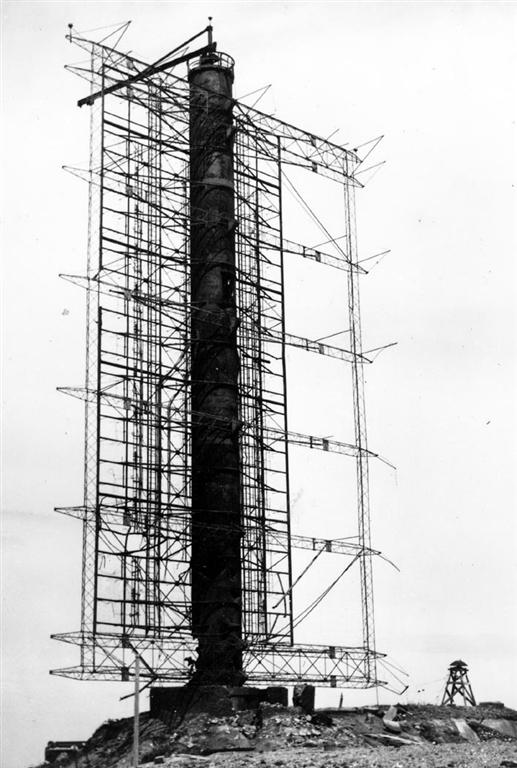
\includegraphics{KHTF.jpg}}
\caption{German Passive Technology, the Klein Heidelberg, 1943 \cite{pic1}}
\label{KH}
\end{figure}

\bigskip

Passive radar technology was starting to come to the forefront, and a number of technological factors were helping. First, the appropriate signal processing power was becoming available to make the system commercially viable. Another contributing factor was the increase in high gain, high signal strength digital broadcasting frequencies, such as digital TV \cite{JE8}. These have helped passive radar stay on the forefront of radar technologies.

\bigskip

As well as these factors, passive radar systems have many advantages over active systems. The main distinguishing factor between passive and active radar is the presence (or lack of in the case of passive), of a transmitting antenna. This leads us to the advantage that passive radar has over active radar, its ability to detect covertly. Not only is this technology covert, but it also is a cost effective counter to stealth. A system of passive receivers can track, detect and target stealth operations, as well as providing information for anti-air systems \cite{Arend}. The system is also more immune to electronic counter measures (ECM), such as jamming from opposition transmitters \cite{HK6}. With all of these features considered, passive radar technology has shown to have very strong military applications. Passive radar has also been used for civilian applications. PARASOL is a project sponsored by the German ministry of environmental affairs that uses passive radar for collision warning of wind power plants \cite{HK5}. It employs a passive radar system that uses the DVB-T illuminators to detect aircraft approaching wind farms and also to reduce the collision of birds.

\bigskip

It has been shown that the predicted detection ranges for a variety of illuminators of opportunity, including analogue FM radio, cellular phone base stations and digital audio broadcast (DAB) is in the order of 'several tens of kilometres' \cite{HD9}. The signals of interest in latest works on the topic have been focused on DVB-T (Digital Video Broadcasting - Terrestrial) signals \cite{gcc,MB11,MC12,MK13}. These signals have a higher transmitter gain and signal power, although the exact medium of the illuminating signal does not have a direct effect on the method of resolving target position and velocity.

\cleardoublepage

\chapter{Background}

\section{Related Work}

Many authors have proposed different methods of solving the problem of resolving the speed and locations of targets using a passive radar system. All system models consist of at least one passive receiver (will be denoted Rx), at least one non-cooperative transmitter or illuminator of opportunity (will be denoted Tx) and at least one target that may be stationary or moving. While these factors remain constant between methods, there are a number of choices that can be made in deriving a model. These include:

\begin{itemize}
\item{Single receiver or multiple receiver}
\item{Using a single illuminator or multi-band/channel illuminators}
\item{Position of transmission source known vs unknown}
\item{Noise variance known vs unknown}
\item{Method for calculating position involves}
	\begin{itemize}
	\item{Correlation between each Tx-Rx pair for computation}
	\item{Correlation between each Rx-Rx pair for computation}
	\item{A combination of both}
	\end{itemize}
\end{itemize}

While these are not the only choices to be made when designing a passive radar system, they are the most common considerations when employing a passive methodology. The big point of difference between many techniques is the algorithm used to detect and track target objects.

\subsection{Problem Set-up}

Many of the techniques follow similar steps to obtain the positions and speeds of targets. Initially a signal model is generated, and received signals are measured for coherence and time delay estimation [14]. To do this, signals need to be time and frequency shifted so they are in the same frame of reference. Doing this requires knowledge of the geometric location of the receivers. If a transmitter generates a signal $s(t)$, the Rx receives a time and frequency shifted version of that signal with noise, namely

\begin{equation}
\label{eqn:approx}
x(t) \approx \mu s(t-\tau) e^{j\omega t} + n(t)
\end{equation}

\bigskip

where $\mu$ is the signal amplitude, $\tau$ is the time delay, $\omega$ is the frequency shift, and $n(t)$ is the noise present in the receiver. This signal can then be time and frequency adjusted, and sampled appropriately to produce a vector

\begin{eqnarray}
\label{eqn:update}
\bar{x}(t) & = & x(t+\tau) e^{-j\omega t} = \bar{\mu} s(t) + \xi(t) \\
\label{eqn:update2}
\bar{x}[n] & = & \bar{\mu}s[n] + \xi[n]
\end{eqnarray}

\bigskip

where $\xi$ represents the time and frequency adjusted noise. The signal $\bar{x}[n]$ is the signal of interest that analysis will be performed on. In practice, we do not know ahead of time what the correcting factors $\tau$ or $\omega$ will be, so we must generate the signals $\bar{x}[n]$ for analysis for each possible time and frequency delay in a multi-dimensional grid. This is discussed further in section~\ref{sec:TFE}.

\bigskip

It is also important to note that if the noise introduced is additive, white, Gaussian noise, that is not dependent on the signal $s(t)$,  equation~\ref{eqn:update2} is correct whether the time and frequency correction occurs before or after the sampling occurs. 

\bigskip

We now need to manipulate these signals to perform some detection analysis, by finding the likelihood that either of the the following two hypotheses are true. This is done by comparing these two hypotheses,

\begin{itemize}
\item{the null hypothesis, where the received signals are simply given by random white gaussian noise}
\item{the alternative hypothesis, where the received signals are correlated due to the signal containing a reflected signal from a target}
\end{itemize}

\bigskip

These are compared by a metric known as the generalised likelihood ratio test (GLRT). This is the real distinguishing factor between methods, and there are a number of approaches of interest to this project, including:

\begin{itemize}
\item{Generalised Canonical Correlation analysis (GCCA) for a single transmitter \cite{gcc}}
\item{Bayesian detection for signals of know rank with known and unknown noise variance \cite{SS15}}
\item{Source localisation for each Rx-Rx pair and each Tx-Rx pair \cite{DE16}}
\item{Using single frequency network analysis for detection \cite{SFN}}
\end{itemize}

\bigskip

This metric is then calculated over a multi-dimensional array, spanning two spatial directions and multiple frequencies. In practice, it is usually viewed as a 2-D spatial grid for each frequency. This gives us a physical view of the likelihood of a target occurring at each position in an image known as the plan position indicator (PPI) map. Some images of PPI maps appear in the Implementation section~\ref{gccaI}. Some methods also include post analysis on the PPI map, for a sharpened location of targets.

\subsection{Generalised Canonical Correlation Analysis}
One such method for determining a GLRT is using Generalised Canonical Correlation Analysis \cite{gcc}.
This method determines the likelihood based on a method that is analogous to generalised canonical correlation in multivairate stasitcs. 

\bigskip

It is easiest to first analyse the case where there exists only two receivers, and then extend the results. Consider the two receiver case, where the received signals are $x_{1}(t)$ and $x_{2}(t)$, and the transmitter broadcasts a signal $s(t)$. Then, as above in equation \ref{eqn:approx}, we know that the received signals are time and frequency shifted.

\begin{eqnarray}
x_1(t) & \approx & \mu_1 s(t-\tau_1) e^{j\omega_1 t} + n_1(t) \\
x_2(t) & \approx & \mu_2 s(t-\tau_2) e^{j\omega_2 t} + n_2(t)
\end{eqnarray}

\bigskip

Here we know that the scalars $\mu_i$ and $\tau_i$ are different, because the receivers are spatially separated, resulting in different time delays and isotropic signal decay. The $\omega_i$ are different for the same reason, but this will be explained further in section ~\ref{sec:doppler}.

\bigskip

Again, as in equation ~\ref{eqn:update}, we can correct for the time and frequency at a given hypothesis location (See section ~\ref{sec:TFE}) by

\begin{eqnarray}
\bar{x_1}(t) & = & x(t+\tau_1) e^{-j\omega_1 t} = \bar{\mu_1} s(t) + \xi_1(t) \\
\bar{x_2}(t) & = & x(t+\tau_2) e^{-j\omega_2 t} = \bar{\mu_2} s(t) + \xi_2(t)
\end{eqnarray}

\bigskip

Now if we take $N$ samples from each of these $\bar{x_i}$ signals, and we know the signal noise variance $\sigma^2$, we can calculate the likelihood that $s(t)$ was our transmitted signal, given that we know the corrected $\bar{x_1}$ and $\bar{x_2}$. We must also consider the relative signal amplitudes, $\mu_1$ and $\mu_2$ in this calculation. This gives us the following likelihood

\begin{equation}
L(\mu_1,\mu_2, s | \bar{x_1}, \bar{x_2}) = \frac{1}{(2\pi\sigma^2)^N} \exp{
\Bigg(- \frac{\| \bar{x_1}-\mu_1 s\|^2 + \| \bar{x_2}-\mu_2 s\|^2}{2\sigma^2} \Bigg)}
\end{equation}

\bigskip

We now wish to maximise this likelihood. Taking the log of this does not effect the maximisation process, so we can develop the log-likelihood

\begin{equation}
l(\mu_1,\mu_2, s | \bar{x_1}, \bar{x_2}) = \log{\Bigg(\frac{1}{(2\pi\sigma^2)^N}\Bigg)}
- \frac{\| \bar{x_1}-\mu_1 s\|^2 + \| \bar{x_2}-\mu_2 s\|^2}{2\sigma^2}.
\end{equation}

\bigskip

Here we have some constant terms that can be ignored for the sake of maximisation. This gives us our simplified log-likelihood

\begin{equation}
l(\mu_1,\mu_2, s | \bar{x_1}, \bar{x_2}) = - \| \bar{x_1}-\mu_1 s\|^2 - \| \bar{x_2}-\mu_2 s\|^2.
\end{equation}

\bigskip

We wish to simplify this further. We can maximise $l$ further by conditioning it only on $s$, by setting

\begin{eqnarray}
\mu_1 & = & \frac{s^\dagger \bar{x_1}}{\|s\|^2} =  \frac{s^\dagger \bar{x_1}}{s^\dagger s}\\
\mu_2 & = & \frac{s^\dagger \bar{x_2}}{\|s\|^2} =  \frac{s^\dagger \bar{x_2}}{s^\dagger s}
\end{eqnarray}

\bigskip

where $.^\dagger$ denotes the complex conjugate. Substituting this into $l$, we can eliminate $\mu_1$ and $\mu_2$ from the likelihood equation.

\begin{equation}
l(s | \bar{x_1}, \bar{x_2}) = - \bigg\| \bar{x_1}-\frac{ss^\dagger }{s^\dagger s} \bar{x_1} \bigg\|^2
- \bigg\| \bar{x_2}-\frac{ss^\dagger }{s^\dagger s} \bar{x_2} \bigg\|^2
\end{equation}

\bigskip

This can then be expanded, and after cancelling terms, yields

\begin{equation}
\label{eqn:const}
l(s | \bar{x_1}, \bar{x_2}) = - \bar{x_1}^\dagger \bar{x_1} - \bar{x_2}^\dagger \bar{x_2}
+ \frac{s^\dagger F s}{s^\dagger s}
\end{equation}

\bigskip

where

\begin{equation}
F = \bar{x_1}\bar{x_1}^\dagger + \bar{x_2}\bar{x_2}^\dagger = \Phi \Phi^\dagger
\end{equation}

\bigskip

and $\Phi$ is the $N\times2$ matrix given by $(\bar{x_1} \bar{x_2})$. Now the first two terms on the RHS of equation~\ref{eqn:const} are constant for any given $\bar{x_i}$, so can be ignored for the maximisation problem. So maximising the likelihood becomes the same as maximising the remaining Rayleigh Quotient term.

\medskip

The maximum value of this quotient is given by the largest eigenvalue in the matrix $F$. Now this matrix is given by $\Phi \Phi^\dagger$ and so is an $N\times N$ matrix. However, it is also true that the largest eigenvalue of the $F$ matrix is also equal to the largest eigenvalue of the matrix $G = \Phi^{\dagger} \Phi$. This matrix $G$ is known as the Gram matrix, or the covariance matrix. For the case of two receivers, this is a $2\times2$ matrix, so computing the eigenvalues of $G$ is much simpler.

\bigskip

Extending this idea to the case with arbitrary number of receivers, we can again form a matrix $\Phi$, by taking the time and frequency corrected signals from each of the receivers, and and placing them into each column. So the amalgamated signals look like $\Phi = (\bar{x_1} \bar{x_2} \ldots \bar{x_r} )$ when there are $r$ receivers. The $r\times r$ Gram matrix is then calculated, and the largest eigenvalue of this is computed. This is the GLRT value that is used in the PPI map.

\section{Theory}

\subsection{Time and frequency estimation}
\label{sec:TFE}
As mentioned above, all of these methods rely on some procedure for estimating the time and frequency delays of the received signals. Since these are not known ahead of time, we must derive these based on our guesses for the position and frequency of the targets.

\bigskip

The first question is what range can be expected from the receivers. We can determine the distance to the horizon by \cite{RHB}

\begin{equation}
D_{h} = \sqrt{2 \times H \times R_{e}}
\end{equation}

\bigskip

where $D_{h}$ is the distance to the horizon in kilometres, $H$ is the height of your receiver in kilometres, and $R_{e}$ is the radius of the earth in kilometres and is equal to $6.4\times 10^{3}$ km. This formula does not take into account refraction off the atmosphere, but for the purposes of passive radar detection, any signals that are refracted in this manner are going to be too weak to be useful. If we assume a receiver height of 30 m, we find that we have a distance to horizon of 19.6 or roughly 20 km. This is the value that will be used.

\bigskip

Next the spatial steps need to be determined. This calculation will determine the resolution that the Plan Position Indicator map will have, and is related to the sampling frequency of the receiver, $f_{s}$. The maximum distance travelled by a wave between samples is given by 

\begin{equation}
D = \frac{C}{f_{s}}
\end{equation}

\bigskip

where $C$ is the speed of light through air. We will be working with receivers that have a sampling frequency of 8 MHz, so the maximum distance travelled between consecutive received samples is around 37.5 m. So to get maximum possible resolution and range, there must be a calculation performed for every 37.5 m block in the x- and y-directions, up to a distance of 20 km from the receiver. In other words, if a receiver is located at the origin of a Cartesian coordinate system, we must take analyse the set of points found by a grid bounded by (-20 000, -20 000), (-20 000, 20 000), (20 000, 20 000), and (20 000, -20 000), with 37.5 m spacings.\footnote{This is a simplification of the scenario that aids in computation. If you wished to be more precise with the domain, you would consider a circle of radius 20 000 m centred on the origin.} 

\bigskip

If the relative locations of the transmitter and receiver are known, the time delay between the direct path signal and the theorised target path signal can be calculated. Let $P_{tx}$ be the position of the transmitter, $P_{rx}$ be the position of the receiver, and $P_{T}$ be the theorised position of the target. Then

\begin{eqnarray}
\label{eqn:dtxrx}
D_{tx\colon rx} & = & \| P_{tx} - P_{rx} \| \\
\label{eqn:dtxtrx}
D_{tx\colon T\colon rx} & = & \| P_{tx} - P_{T} \| + \| P_{T} - P_{rx} \| \\
\label{eqn:PD}
D_{ \textnormal{Path Difference}} & = & D_{tx\colon T\colon rx} - D_{tx\colon rx}
\end{eqnarray}

\bigskip

Now the path difference, coupled with the sampling frequency can tell us exactly how many samples the direct path, and target path signals are expected to be delayed by. The time taken for a signal to travel a distance $D_i$ is given by 

\begin{equation}
t_i = \frac{D_i}{C}
\end{equation}

\bigskip

To convert this to a digital delay in samples, we again need to know the receivers sampling frequency, $f_s$. Now the number of samples it is delayed by, is simply given by

\begin{equation}
N_i = t_i \times f_s.
\end{equation}

\bigskip

So, to do time estimation, we simply need to delay each of the received signals by the correct number of samples, dependent only on the distance from the estimated target.

\bigskip

The next element that must be considered is frequency shifting. Frequency shifting is important because most targets of interest will be moving, and have a Doppler shift relative to the receiver. If this Doppler is not accounted for, the detection method will not be able to detect the reflected signals off the target because the signals at different receivers will not be frequency synchronised.

\bigskip

If we wish to shift a signal by our estimated frequency, $f_x$ (note that this frequency shift can be positive or negative), we must first create a time vector that corresponds to our samples. To do this, we simply take the sampling period

\begin{equation}
T = \frac{1}{f_s},
\end{equation}

\bigskip

and create a vector of times $t_v = \{0, T, 2T, \ldots , (N-1)T\}$ that is the same length as our received signal (ie $N$ samples). Then if $x(t)$ is our unshifted signal, we can obtain our shifted signal by 

\begin{equation}
\hat{x}(t) = x(t) \times \exp (2\pi i f_x t_v )
\end{equation}

\bigskip

where $\hat{x}(t)$, $x(t)$, and $t_v$ are all column vectors and the multiplication is performed element wise. This produces our frequency shifted signal that we can now perform analysis on.


\subsection{Range-Doppler Maps}
\label{sec:rdMap}
Range-Doppler maps are another important idea in the development of this thesis. They are essentially another way of displaying the information about targets surrounding a receiver. They do not, however, present this information in the spatial domain, as the PPI maps do. Instead they display information in the Range-Doppler domain. 

\bigskip

In this domain, the range axis represents the path difference (see equation \ref{eqn:PD}) between a direct path, and a target path. The direct path (equation~\ref{eqn:dtxrx}) is the path directly from the transmitter to the receiver, while the target path (equation~\ref{eqn:dtxtrx}) refers to any path from the transmitter, to a target, then to the receiver.

\bigskip

Expectantly, the Doppler axis refers to the Doppler shift that the signal experiences when it hits a moving target. Further explanation of how and why this occurs is found in section ~\ref{sec:doppler}. An example of what a Range-Doppler map looks like appears in figure~\ref{fig:rdm1}.

\bigskip

Calculation of the Range-Doppler domain is rather simple. The received signal, $x(t)$, is correlated with a time and frequency shifted version of itself,

\begin{equation}
\hat{x}(t) = x(t-\tau) e^{ -2\pi i f_x t}.
\end{equation}

\bigskip

Here, again $\tau$ is our time shift and $f_x$ is our frequency shift. The value of the correlation of these two signals, $\textnormal{corr}(x,\hat{x})$, is then placed at the grid point in the Range-Doppler map corresponding to the correct time and frequency shifts.

\bigskip

The peaks in this plot will occur at the points where a target is located.
If we consider the case where the broadcast signal is $s(t)$, the received signal from the direct path is $\mu_1s(t-\tau_1)$, and the signal from one of the target paths is $\mu_2s(t-\tau_2)e^{2\pi i f_x t}$. We know the correct time shift for the Range, or more correctly, path difference, is given by\footnote{Note that the actual shift is $\tau_2 - \tau_1$. However, we are accounting for, and trying to undo this shift, so we must take the negation of it, $\tau_1 - \tau_2$.} $\tau_1 - \tau_2$, and the correct frequency shift is $f_x$, then we can calculate that

\begin{eqnarray}
\label{eqn:x1}
x(t) & = & \mu_1s(t-\tau_1) + \mu_2s(t-\tau_2)e^{2\pi i f_x t} \\
\hat{x}(t) & = & x\bigg(t-(\tau_1 - \tau_2)\bigg) e^{ -2\pi i f_x t} \\
 & = & \mu_1s\bigg(t-(\tau_1 - \tau_2)-\tau_1\bigg)e^{ -2\pi i f_x t}	 + \mu_2s\bigg(t-(\tau_1 - \tau_2)-\tau_2\bigg) \\
 \label{eqn:x2}
  & = & \mu_1s(t-2\tau_1 + \tau_2)e^{ -2\pi i f_x t} + \mu_2s(t-\tau_1)
\end{eqnarray}

\bigskip

Here we can see that the first term in equation~\ref{eqn:x1} and the last term in equation~\ref{eqn:x2} share a common function, $s(t-\tau_1)$. This means that the correlation of $x$ and $\hat{x}$ will be higher than for other shifts not having this commonality.

\bigskip

It is also worth noting that the signal $x$ and $\hat{x}$ both contain complex values, so the resulting correlation value will also be complex. Ideally a singe real value for each hypothesis point is needed. Just taking the real part of the correlation is ignoring half of the data, and creates some unwanted behaviour near the origin of the Range-Doppler map. To avoid this, the absolute value of the correlation is taken and used.

\bigskip

This is not the only unwanted behaviour of this method. There are also some shadows that appear in the Range-Doppler map that do not correspond with targets. These shadows are artefacts caused by the correlation of the other terms of $x$ and $\hat{x}$. This and the unwanted behaviour near the origin is due to the signal noise being correlated with itself.

\bigskip

Better radar receivers can be tuned to receive only a direct path signal. These are known as omni-directional antennas. These antennas can actually receive two signals, a direct path only signal $d(t)$ and a non-directional signal $n(t)$. We can improve the behaviour of the Range-Doppler method by using one of these antennas and taking the correlations between $d(t)$ and the time and frequency corrected versions of $n(t)$.

\bigskip

This improves the response at the origin as well as removing any artefacts that would have occurred with the other method. We know this because we are now always correlating with the direct path signal, and not a mix of cross-terms that may be correlated at other places.

\bigskip

The correlation of two complex signals $x[n]$ and $y[n]$ is strictly defined as

\begin{equation}
R_{xy}(0) = \sum_{m=-\infty}^{\infty} x[n] y^*[n-m]
\end{equation}

\bigskip

When we have finite signals, the bounds are smaller, but we still need to calculate all of the inner product terms. Doing this naively can be quite computationally expensive. However, there is a simpler way to do this through Fourier Transforms. The Weiner-Khintchine theorem tells us that 

\begin{equation}
\mathcal{F} \bigg(R_{xy}(\tau) \bigg) = G_{xy}(f)
\end{equation}

\bigskip

Where $\mathcal{F}$ denotes the Fourier transform, and $G_{xy}(f)$ is the energy cross spectral density of $x$ and $y$. This cross spectral density can also be calculated as 

\begin{equation}
G_{xy}(f) = \mathcal{F}(x) \bigg(\mathcal{F}(y)\bigg)^*
\end{equation}

\bigskip

So a faster method to calculate the correlation of two signals is given by

\begin{equation}
R_{xy} = \mathcal{F}^{-1} \Bigg( \mathcal{F}(x) \bigg(\mathcal{F}(y)\bigg)^* \Bigg)
\end{equation}

\bigskip

where $y$ is our direct path only signal, and $x$ is our frequency corrected signal. Here we can use the fast Fourier Transform (FFT) algorithm to calculate the correlations in $O (n \log n)$ time. Another bonus of doing this, is that it calculates all of the cross correlations at once, so we do not need to do any time shifting. This time-shifting happens automatically in the FFT algorithm.

\subsection{Radar Cross Section and Radar equation}
\label{sec:RCSeqn}
Any analysis of radar would be remiss not to mention the Radar Cross Section (RCS) equation. This equation is a measure of how detectable an object is with a radar. The idea is to determine the cross-sectional area that hits a radar target to determine the isotropic spread of the signal. The radar equation is given by

\begin{equation}
\label{eqn:rcs1}
P_r = \frac{P_tG_tG_rA_{eff}}{4\pi d^2}
\end{equation}

\bigskip

where $P_r$ and $P_t$ are the power received and transmitted respectively (measured in Watts), $G_r$ and $G_t$ are the respective gains of the receiver and transmitter (as scalars), $A_{eff}$ is the effective area of the radar antenna (in metres squared), and $d$ is the distance between the receiver and transmitter (in metres).

\bigskip

This equation will be relevant when calculating the scaling value $\mu$ for the direct path signal. Here we would simply substitute in the know values for $P_t,G_t,G_r,A_{eff}$ and use $D_{tx\colon rx}$ as the value for $d$. The simulations, however, use signal amplitude, rather than power. So we need to relate these two using the known relation

\begin{equation}
A = \sqrt{2P}
\end{equation}

\bigskip

Substituting this into the equation~\ref{eqn:rcs1} gives

\begin{eqnarray}
A_r &=& \frac{A_t}{d} \sqrt{\frac{G_tG_rA_{eff}}{4\pi}} \\
\label{gain1}
A_r &=& \frac{A_t}{d} G,
\end{eqnarray}

\bigskip

where $A_r$ and $A_t$ are the amplitudes at the receiver and transmitter respectively and $G$ is a constant that encompasses all of the scalar gains of the system.

\bigskip

The other consideration is how to treat signals that bounce off a target and head towards a receiver. Let a target be located at a distance of $d_1$ from the transmitter and $d_2$ from the receiver. Then the strength of the signal at the target is given by substituting $d_1$ into equation~\ref{eqn:rcs1}. Now the target acts as its own receiver and re-broadcasts the signal at this lower strength. This reflected signal is then isotropically radiated outwards. Substituting in this Radar cross section term\footnote{$\sigma$ is measured in metres squared and is given by the cross sectional area of the target with respect to the transmitter} $\sigma$ into the radar equation, we can determine the power received from this signal at the receiver by

\begin{equation}
\label{eqn:rcs2}
P_r = \frac{P_tG_t}{4\pi d_1^2} \sigma \frac{G_r}{4\pi d_2^2}A_{eff}
\end{equation}

\bigskip

Again we can move this into an equation relating to amplitude rather than power, yielding

\begin{eqnarray}
A_r &=& A_t \sqrt{\frac{G_t}{4\pi d_1^2} \sigma \frac{G_r}{4\pi d_2^2}A_{eff}} \\
A_r &=& A_t \sqrt{\frac{G_tG_r\sigma A_{eff}}{(4\pi)^2d_1^2d_2^2}} \\
A_r &=& \frac{A_t}{d_1d_2} \sqrt{\frac{G_tG_r A_{eff}}{4\pi}} \sqrt{\frac{\sigma}{4\pi}} \\
\label{eqn:add}
A_r &=& \frac{A_t}{d_1d_2} G \Sigma.
\end{eqnarray}

\bigskip

Here $G$ is the same gain constant used above in equation~\ref{gain1}, and $\Sigma$ is a constant that relates only to the cross-sectional area of the target. Targets with a higher RCS will be easier to identify, because they radiate more of the transmitted signal through reflection than smaller targets.

\bigskip

The gain constant $G$, the RCS constant $\Sigma$, and the SNR (see section~\ref{sec:snr}) are the parameters used to estimate the channel that the signals are being broadcast in. The two parameters mentioned in this section are given by

\begin{eqnarray}
G &=& \sqrt{\frac{G_tG_r A_{eff}}{4\pi}}\\
\Sigma &=& \sqrt{\frac{\sigma}{4\pi}}
\end{eqnarray} 

\subsection{Doppler Shift}
\label{sec:doppler}
The Doppler effect is the change in frequency of a wave due to the relative velocities of the source and observer. Bistatic Doppler shift is a specific example of the Doppler effect, present in systems with spatially separated transmitters and receivers, such as in Passive Radar. It can be thought of as the rate of change of the bistatic range, $D_{tx\colon T\colon rx}$, from equation~\ref{eqn:dtxtrx}. Alternatively, it can be given by

\begin{equation}
f_{\textnormal{shift}} = \frac{1}{\lambda} \frac{d}{dt}\bigg( R_{tx} + R_{rx} \bigg),
\end{equation}

\bigskip

where $f_{\textnormal{shift}}$ is the frequency that the signal is shifted by, $\lambda$ is the transmitted signals wavelength, and $R_{tx}$ and $R_{rx}$ are the distances from the target to the transmitter and receiver respectively. The derivative terms can be approximated by taking the projection of the velocity of the target onto the straight line joining the target to the receiver or transmitter.

\bigskip

Let the target of interest have velocity $V = (v_x,v_y)$, and the transmitter, receiver and target be located at $P_{tx}$, $P_{rx}$, and $P_T$ respectively. Then we can approximate the derivatives by

\begin{eqnarray}
\frac{dR_{tx}}{dt} &=& \frac{V\bullet(P_T - P_{tx})}{\|P_T - P_{tx}\|} \\
\frac{dR_{rx}}{dt} &=& \frac{V\bullet(P_T - P_{rx})}{\|P_T - P_{rx}\|}
\end{eqnarray}

\bigskip

where $\bullet$ denotes the vector dot product. The final unknown is $\lambda$, the transmitted signals wavelength. This is related to the centre frequency of the transmitted signal. This is the frequency band that the signal is actually broadcast on. It will be denoted by $f_0$ and is nominally 220 MHz for this thesis. The wavelength is related to this vale by

\begin{equation}
\lambda = \frac{C}{f_0}.
\end{equation}

\bigskip

So, we can substitute all of these into the bistatic Doppler equation to get that the frequency shift at the receiver is given by

\begin{equation}
f_{\textnormal{shift}} = \frac{f_0}{C} \Bigg(\frac{V\bullet(P_T - P_{tx})}{\|P_T - P_{tx}\|} +  \frac{V\bullet(P_T - P_{rx})}{\|P_T - P_{rx}\|}\Bigg)
\end{equation}

\bigskip


\subsection{Signal to Noise Ratio}
\label{sec:snr}
The final point of interest is the signal to noise ratio (SNR). This is the ratio of signal power to noise power present in the received signal and is a measure of how clean the received signal is. It is usually measured in dB. Higher SNR means that the meaningful information in the signal is more prevalent than the random noise. The noise that occurs in receivers is random Gaussian white noise due to thermal components. The power of this noise is given by the variance of the noise, so we can generate a noisy channel with arbitrary SNR given a known, clean signal. The equations relating SNR quantities are

\begin{equation}
\textnormal{SNR} = \frac{P_{\textnormal{signal}}}{P_{\textnormal{noise}}} = \frac{\sigma_{\textnormal{signal}}^2}{\sigma_{\textnormal{noise}}^2} = \Bigg(\frac{A_{\textnormal{signal}}}{A_{\textnormal{noise}}} \Bigg)^2
\end{equation}

\bigskip

Note that the above formula uses the linear SNR. We will almost exclusively work in dB, so to convert between the two, you simply need

\begin{equation}
\textnormal{SNR}_{\textnormal{DB}} = 10 \log_{10}\textnormal{SNR}
\end{equation}

\bigskip

Typical SNR values for radar receiver systems can occur anywhere between -10 and 50 dB, depending on the characteristics of the channel through which the signal is propagating\cite{SNR}. This value can be greatly affected by temperature, and is known as thermal noise \cite{thermal}.

\begin{figure}[p]
\centering
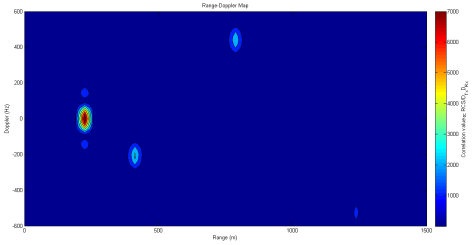
\includegraphics{RDMAP2.png}
\caption{Range-Doppler Map with 4 targets}
\label{fig:rdm1}
\end{figure}


\cleardoublepage

\chapter{Implementation of prior works}

Before trying to develop a new method, it was important to first implement some of the previous methods that had been used to solve the problem. This posed a number of challenges, and the solutions to these were used as the code base for the rest of the thesis.

\section{Simulating Signals}
The first challenge in implementing a passive detection system, is simulating the environment that the signals are being transmitted in. There are many factors that must be accounted for to create a realistic simulation.
The simulations used in this thesis take into account the following factors

\begin{itemize}
	\item{Relative positions of transmitter, receivers, and targets}
	\item{Sampling frequency of the receiver and carrier frequency that is being broadcast}
	\item{Signal to noise ratio at the receivers}
	\item{Radar cross section of targets and radar equation}
	\item{Doppler shift due to targets velocity}
\end{itemize}

Explanation of how these are incorporated into the simulation design can be found below. The code listing for the signal generation can be found in appendix~\ref{app:siggen1}.

\subsection{Generating Signals}
When the simulation is run, it must generate a number of signals for the transmitter to broadcast. In reality, these are the signals that a digital TV, or radio station would be broadcasting. Due to the nature of the transmission schemes used, these signals will be complex, with zero mean. These signals were simulated as complex, Gaussian random variables with zero mean and unitary variance. This can be done simply in MATLAB, with the command:

\begin{verbatim}
                   S = randn(Ngen,1) + 1i*randn(Ngen,1);
\end{verbatim}

Where \verb+S+ is the signal the transmitter broadcasts, and \verb+Ngen+ is the number of samples we wish to generate. This \verb+S+ is then used to generate all of the received signals.

\bigskip

The format of the received signals, will be an $n\times r$ matrix, $\Phi$, where $n$ is the number of samples of the received signal, and $r$ is the number of receivers. Each column of the $\Phi$ matrix corresponds to the received signals at a receiver.

\subsection{Relative Positions}
The relative positions of the transmitter, receivers, and targets is the most important factor in developing this simulation. As mentioned in the \ref{sec:TFE}, we can define the distance $D_{tx\colon rx}$ (see equation~\ref{eqn:dtxrx}) for each receiver. We can also define for each receiver-target pair, the distance $D_{tx\colon T\colon rx}$ (see equation~\ref{eqn:dtxtrx}). 

\bigskip

Initially, each receiver will be given the direct path signal from the transmitter. This is calculated by shifting the generated signal \verb+S+ by $N_{\textnormal{Shift1}}$ samples, defined by

\begin{equation}
N_{\textnormal{Shift1}} =
\bigg\lfloor  \frac{D_{tx\colon rx}}{C} f_s \bigg\rfloor
\end{equation}

\bigskip

where $C$ is the speed of light in air and $f_s$ is the sampling frequency of the receiver. Each receiver will also receive a signal emanating from each target. This signal will again be a scaled version of the generated signal \verb+S+, this time shifted by

\begin{equation}
N_{\textnormal{Shift2}} =
\bigg\lfloor  \frac{D_{tx\colon T\colon rx}}{C} f_s \bigg\rfloor
\end{equation}

\bigskip

This second received signal will also have a frequency shift associated with it, dependent on the target's velocity, which is accounted for in section ~\ref{FS}. Both of these signals will also be scaled appropriately, as discussed in section ~\ref{RE}.

\subsection{Radar Equation}
\label{RE}
This section directly references material covered in section~\ref{sec:RCSeqn}. The implementation of these aspects was a direct implementation of the theory. A section of the code that appears in appendix~\ref{app:siggen1} is shown below to demonstrate this implementation.


\begin{verbatim}
% Give each receiver the signal from each target and transmitter
for trans = 1:ntx
    for rec = 1:nrx
        for targ = 1:ntarg
            R1 = DTxTarg(trans,targ);
            R2 = DRxTarg(rec,targ);
            DIST = R1 + R2;
            TIME = DIST / C;
            SAMP = round(TIME / dt);
            %Get the signal and frequency correct it
            sig = S.*exp(1i*2*pi*FShift(trans,rec,targ)*timevec);
            %Get the correct part of the signal (wrt time)
            sig = sig(1:Ngen-SAMP+1); 
            AMP = GAIN*SIGMA / (R1*R2); %Signal amplitude
            phi(SAMP:end,rec) = phi(SAMP:end,rec) + AMP*sig;
        end
    end
end
\end{verbatim}

The line \verb+AMP = GAIN*SIGMA/(R1*R2)+ relates directly to the constants $G$ and $\Sigma$ mentioned in section~\ref{sec:RCSeqn}. A similar code snippet exists for the direct path signal, although is slightly simpler.

\subsection{Frequency Shift}
\label{FS}
The frequency shift was discussed in section~\ref{sec:doppler}. A simple implementation of this appears in the code snippet below.

\begin{verbatim}
timevec = 0:dt:dt*(Ngen-1);
timevec = timevec';
sig = S.*exp(1i*2*pi*FShift*timevec);
\end{verbatim}

Here \verb+Ngen+ is the length of the non frequency shifted signal, \verb+S+. \verb+Fshift+ is the desired frequency shift, and \verb+sig+ is the resulting vector. The value \verb+dt+ is the period of the sampling rate and is equal to $\frac{1}{f_s}$.

\section{GCCA Implementation}
\label{gccaI}
The full code for the implementation of the GCCA algorithm appears in appendix~\ref{app:gcca}. The pseudo code for the algorithm is as follows

\begin{alltt}
for x in xrange
    for y in yrange
        for f in freqrange
            for each receiver r
                d \(\gets\) distance from r to (x,y)
                n \(\gets\) d/C \(\times f\sb{s}\)
                sig1 \(\gets\) signal received at r
                sig2 \(\gets\) sig1 time shifted by n samples
                sig3 \(\gets\) sig2 frequency shifted by f                
                phi(r) \(\gets\) sig3
            end
            G = phi \(\times\) phi' (transpose)
            PPI(x,y,f) = max(eig(G))
        end
    end
end
\end{alltt}

This is the naive implementation of the algorithm. The output of this algorithm is a PPI map.

\bigskip

Let there be five receivers located at $(x,y) = \{(0,0), (0,50), (0,-50), (-50,0), (50,0)\}$, two stationary targets at $(x,y) = \{(100,-150), (20, 100)\}$, and one transmitter located at $(x,y) = (1000,0)$. We can simulate this scenario and develop a PPI map using the GCCA algorithm.  The calculated PPI map for this situation appears in figure~\ref{ppi1}.

\begin{figure}[htbp]
\centerline{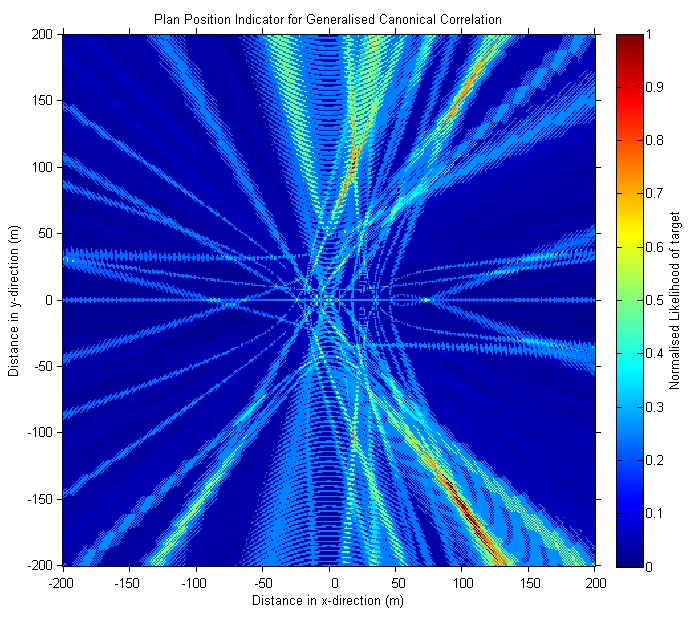
\includegraphics{ppi1.jpg}}
\caption{PPI indicator map for scenario detailed in section~\ref{gccaI}}
\label{ppi1}
\end{figure}

\subsection{Target Detection in PPI map}
Further investigations found that it was possible to extract the locations of the targets from the PPI map with known noise variance. This was done by using a series of image processing techniques and thresholding, the code for which appears in appendix~\ref{IP}.

\bigskip

The PPI map has image dilation performed upon it using a disk structured element, and then converted to black and white using an appropriate threshold. The connected components of this threshold image are then computed, and if their area is above another threshold, they are deemed to be a target. The centre of the pixels in such connected components is then given as the location of the target. This procedure was applied to the same scenario as above, and the results are shown in figure~\ref{ppiip}.

\begin{figure}[htbp]
\centerline{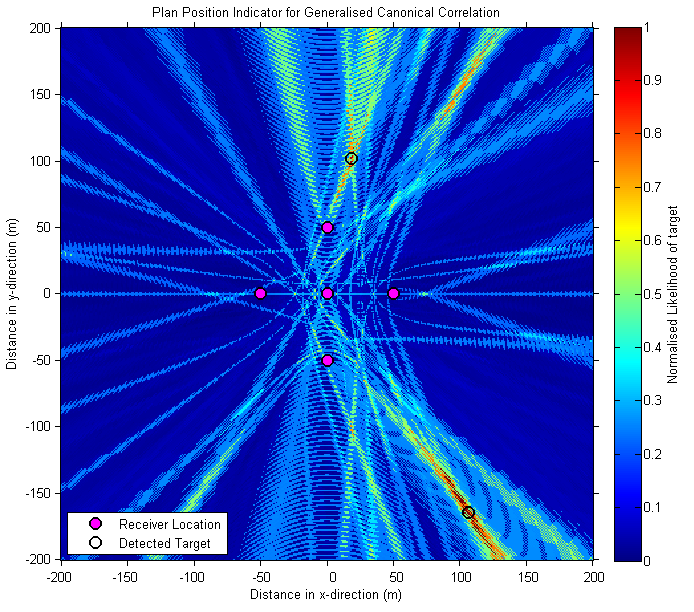
\includegraphics{ppiip.png}}
\caption{PPI indicator map for scenario detailed in section~\ref{gccaI}, with target detection applied}
\label{ppiip}
\end{figure}

\section{Optimisation}


\subsection{Eigenvalue calculation}
The largest eigenvalue computation needs to be performed on a large array of positions and frequencies, so must be done as efficiently as possible. Many different algorithms exist for computing eigenvalues of matrices. The algorithms of interest would need different properties depending on which passive radar method they were applied to. All would need to have a fast convergence rate to be considered appropriate for implementation in a real-time system. There are a number of iterative methods that could be employed, and have been employed for a variety of applications including Power iteration, Rayleigh-quotient iteration and the Lanczos algorithm – for computing eigenvalues \cite{CV17,RA18,IE19}.

\bigskip

A method that was trialled in this thesis is the power method for calculating the largest eigenvalue. This method requires a guess for the largest eigenvalue, and then converges towards it using iterative steps. When then difference between iterations falls below a threshold, the algorithm is said to have converged. This iterative method could use the previously calculated maximum eigenvalue as the initial guess for the next calculation. It was posited that this would speed up calculation of the largest eigenvalue.

\bigskip

However, it was found that the built-in command \verb+eig()+ in MATLAB, was far superior timewise than any m-file implementation of an iterative algorithm. This was especially the case when considering small numbers of receiver, and therefore small matrices.

\subsection{Range-Doppler Usage}
The GCCA method can also be sped up by using the Range-Doppler transformations to calculate the GLRT. This did not become apparent until after the new method had been developed, so is not explored further in this thesis.


\section{Time Complexity}
\label{sec:timecomp}
Finally, an analysis of the time complexity of this algorithm was performed. It is important to note that this is not a fully optimised version of the algorithm, but the version the author was able to implement.

\bigskip

We can let the number of radar receivers be $r$, the maximum scanning range in both the x- and y-directions be $x$, the number of frequency shifts to check be $f$, and the number of samples taken in a time frame be $n$. The number of times the inner for loop in section~\ref{gccaI} is $O(x^2f)$.

\bigskip

In this inner loop, we must copy the time and frequency corrected values of the signals. There are $n$ samples so this takes $O(n)$ time. We must also perform the multiplication $G = \Phi^\dagger \Phi$. Now we know that $\Phi$ is an $n\times r$ matrix, so performing this calculation naively\footnote{For non-square matrices, naive multiplication is close to the best case time complexity.} will take $O(nr^2)$ time. We must finally calculate the largest eigenvalue of our $r\times r$ matrix $G$. This will take $O(r^3)$ time. So we find that the time complexity for the inner loop is given by

\begin{eqnarray}
t_{\textnormal{inner}} &=& O(n + nr^2 + r^3)\\
&=& O\bigg( n(r^2 + 1) + r^3 \bigg) \\
&=& O\bigg( nr^2 + r^3 \bigg) \\
&=& O\bigg( r^2 (n + r) \bigg) \\
\end{eqnarray}

In general we know that $r \ll n$, because the number of receivers is small compared to the number of samples taken. So $O(n + r)$ will always simplify to $O(n)$. So we have the time complexity of the inner loop being

\begin{equation}
t_{\textnormal{inner}} = O\bigg( nr^2 \bigg)
\end{equation}

This means that the total time complexity for the naive implementation of the GCCA algorithm for solving the passive radar detection problem is

\begin{equation}
\label{eqn:time1}
O\bigg(x^2f nr^2 \bigg)
\end{equation}

\cleardoublepage

\verb+ +
\cleardoublepage

\chapter{Design}

\section{Motivation}
The main motivation behind a new approach for passive radar detection stems from the fact that the cost of radar receivers is beginning to fall, as antenna and receiver technology gets cheaper and more efficient \cite{CMOS,lowCost}. This means that it is starting to become plausible to have large networks of cheap receivers working together as a detection system.

\bigskip

With this scalability in hardware, comes the need for a massively scalable algorithm for detection. The large scale of such a system presents its own problems that current detection methods will struggle with, such as

\begin{itemize}
	\item{Greater timing and synchronisation issues due to the larger number of receivers}
	\item{The need to amalgamate all the data at a centralised location for processing}
	\item{The computing power to calculate the PPI map using all of the received data}
\end{itemize}

The current methods all require that the raw received data be sent and synchronised to a high degree of accuracy to the same place for processing. The main focus is to develop an algorithm that is robust to the factors mentioned above and very efficient, as it must scale well.


\section{The Range-Doppler Transformation}
The main idea behind this technique for the Passive Radar detection problem is that signals received at each receiver can be processed separately. The general process for the algorithm is as follows.

\begin{enumerate}
	\item{For each receiver, a Range-Doppler Map is calculated for each predetermined time interval}
	\begin{itemize}
		\item{This calculation is performed at the receiver, meaning less time synchronisation problems}
		\item{This is a simple calculation that utilises the FFT algorithm, as mentioned in section~\ref{sec:rdMap}}
	\end{itemize}
	\item{The target points are detected in the Range-Doppler domain}
		\begin{itemize}
		\item{These points occur as the range-frequency double $(r,f)$}
		\item{This process is shown in section~\ref{sec:detectT}}
	\end{itemize}
	\item{The pair $(r,f)$ in the Range-Doppler domain corresponds to an ellipse in the spatial domain}
	\begin{itemize}
		\item{The ellipse is made up of all of the points that have the same path difference as $(r,f)$}
		\item{The steps for determining the ellipse parameters appears in section~\ref{sec:ell1}}
	\end{itemize}
	\item{The ellipses are then intersected, generating a number of $(x,y)$ spatial domain coordinates}
	\begin{itemize}
		\item{These spatial domain coordinates are amalgamated into a list}
		\item{Each pair of ellipses can intersect in up to four locations, only one of which can correspond to a target}
		\item{The formula for intersecting ellipses is developed in section~\ref{sec:ell2}}
	\end{itemize}
	\item{A voting and consensus algorithm is used to determine the locations of the targets}
	\begin{itemize}
		\item{The highest voted location above a threshold is deemed to be a target}
		\item{All ellipses corresponding to this point are removed, along with all of their intersection points, and the algorithm continues}
		\item{This continues until all targets have been found, and the highest voted location is below a threshold}
		\item{This process is described further in section~\ref{sec:Vote}}
	\end{itemize}
\end{enumerate}

The full implementation of this algorithm appears in appendix~\ref{app:rdt}. What follows below are the implementation details and logic of many of the steps of the algorithm.

\subsection{Detecting Targets in Range-Doppler domain}
\label{sec:detectT}
Once the Range-Doppler map has been calculated, the next step is to detect the targets in this domain. A lot of time was spent developing a model for target detection. It was believed that simulating a lot of targets for each possible receiver-transmitter location would allow us to model the response of the channel and determine some guaranteed levels for detection. This was also something that would only need to be done once, and would be akin to initialisation of the system.

\bigskip

Each receiver-transmitter pair was simulated with multiple targets at different distances away from the receiver. The compressed range-Doppler map showing the amplitude of the correlation versus time was then calculated. This, expectantly, showed a decaying exponential function. A least squares model was found for this line, and this was initially used as the threshold for a detection metric. An example of one of these plots appears in figure~\ref{fig:detect}.

\bigskip

This was deemed unfeasible later for a number of reasons. Firstly, in reality, different targets would have difference RCS values, so would have different detection characteristics in the Range-Doppler domain. Secondly, the path difference is not the metric that determines signal strength. If we recall equation~\ref{eqn:add} from section~\ref{sec:RCSeqn}, we can see that the scaling is not a function of the range, but a function of the product of the distances of the receiver and transmitter from the target. This means that two identical targets at the same path difference but different location can have different detection characteristics in the Range-Doppler domain.

\bigskip

Ultimately it was decided that a global threshold, above the known noise floor, would be used to determine the detection of targets. There still exists some ambiguity in the Doppler domain, which is governed by the radar ambiguity function. To combat this, all of the frequencies at a particular range were compressed onto each other, by taking the maximum value. In effect, we compressed our 2-D Range-Doppler map into a 1-D Range plot. Peak detection was then performed on this plot to determine the path differences that the targets occurred at. The code implementation for this appears in appendix~\ref{app:tdetect}.

\subsection{Generating ellipse coefficients}
\label{sec:ell1}
Once we have detected the ranges that the targets occur at, we must convert these path differences into ellipse equations in the spatial domain. The transmitter and receiver become the foci of the ellipse, and the range, also known as the path difference, is given by $PF_1 + PF_2 - F_1F_2$, with respect to the ellipse in figure~\ref{fig:ell1}. It is known that

\begin{equation}
PF_1 + PF_2 = 2a
\end{equation}

\bigskip

where $a$ is the major axis length. We know the distance between the the transmitter and receiver, $F_1F_2$, so we can work out this axis length by

\begin{eqnarray}
P_{\textnormal{diff}} &=& PF_1 + PF_2 - F_1F_2 \\
P_{\textnormal{diff}} &=& 2a - F_1F_2 \\
a &=& \frac{P_{\textnormal{diff}} + F_1F_2}{2}
\end{eqnarray}

\bigskip

where $P_{\textnormal{diff}}$ is the detected path difference, and $F_1F_2$ is the distance between the transmitter and receiver. Both of these quantities are known. $a$ is one of the ellipse parameters known as the major axis length. There is another ellipse measurement, $f$, known as the linear eccentricity, and is a measure of the distance from the centre of the ellipse to the foci. The foci are located equidistant from the centre along a straight line, so this parameter is given by

\begin{equation}
f = \frac{F_1F_2}{2}
\end{equation}

\bigskip

There is another relation that is used to determine the minor axis length, $b$, from the linear eccentricity. This is due to Pythagora's theorem, and relates $a$, $b$, and $f$ by

\begin{eqnarray}
f^2 &=& a^2 - b^2 \\
b &=& \sqrt{a^2 - f^2}
\end{eqnarray}

\bigskip

Now we have the major and minor axis lengths of any ellipse with a transmitter and receiver at the foci and a known path difference. 

\bigskip

The general equation for an ellipse with it's centre at $(x,y) = (x_0,y_0)$, and major and minor axis lengths of $a$ and $b$ is given by

\begin{equation}
\frac{(x-x_0)^2}{a^2} + \frac{(y-y_0)^2}{b^2} = 1
\end{equation}

\bigskip

However, our ellipses may be arbitrarily rotated by an angle $\alpha$, that is determined by the physical layout of the system. If the transmitter is located at $(t_x,t_y)$ and the receiver is located at $(r_x,r_y)$, then the ellipse becomes rotated by an angle

\begin{equation}
\alpha = \tan^{-1}\Bigg(\frac{t_y-r_y}{t_x-r_x} \Bigg)
\end{equation}

\bigskip

The equation of this rotated ellipse is

\begin{equation}
\label{eqn:ellrot}
\frac{\bigg((x-x_0)\cos\alpha + (y-y_0)\sin\alpha\bigg)^2}{a^2} + \frac{\bigg((x-x_0)\sin\alpha - (y-y_0)\cos\alpha\bigg)^2}{b^2} = 1
\end{equation}

\bigskip

All of these constants $a$, $b$, and $\alpha$ are known, and $x_0$ and $y_0$ are simply given by the midpoint between the transmitter and receiver.

\begin{eqnarray}
x_0 &=& \frac{t_x + r_x}{2} \\
y_0 &=& \frac{t_y + r_y}{2} 
\end{eqnarray}

\bigskip

This is not, however, a very useful form. Instead, this equation was turned into a bivariate quadratic equation. The form of this is

\begin{equation}
\label{eqn:biv}
Q(x,y) = q_{xx}x^2 + q_{xy}xy + q_{yy}y^2 + q_x x + q_y y + q_0 = 0
\end{equation}

The equation~\ref{eqn:ellrot} was expanded and simplified to match the terms in equation~\ref{eqn:biv}. This was a long algebraic process, so will not appear in full here. The solutions to solving these equations, as well as the implementation details appear in the coded solution in appendix~\ref{app:ellParam}. The parameters are related as follows

\begin{eqnarray}
q_{xx} &=& \Bigg(\frac{\cos\alpha}{a} \Bigg)^2 + \Bigg(\frac{\sin\alpha}{b} \Bigg)^2 \\
q_{yy} &=& \Bigg(\frac{\sin\alpha}{a} \Bigg)^2 + \Bigg(\frac{\cos\alpha}{b} \Bigg)^2 \\
q_{xy} &=& \frac{2\cos\alpha\sin\alpha}{a^2} - \frac{2\cos\alpha\sin\alpha}{b^2} \\
q_x &=& \frac{-2x_0\cos^2\alpha-2y_0\cos\alpha\sin\alpha}{a^2} + \frac{-2x_0\sin^2\alpha+2y_0\cos\alpha\sin\alpha}{b^2} \\
q_y &=& \frac{-2y_0\sin^2\alpha-2x_0\cos\alpha\sin\alpha}{a^2} + \frac{-2y_0\cos^2\alpha+2x_0\cos\alpha\sin\alpha}{b^2} \\
q_0 &=& \frac{(x_0\cos\alpha + y_0\sin\alpha)^2}{a^2} + \frac{(x_0\sin\alpha - y_0\cos\alpha)^2}{b^2} - 1
\end{eqnarray}

\subsection{Intersecting Ellipses}
\label{sec:ell2}
Once all of the receivers have calculated their Range-Doppler maps, detected targets in this domain, and determined the spatial ellipse parameters, these are all sent to a centralised location for processing. Each receiver may have detected multiple targets, so there will be multiple ellipses per receiver.

\bigskip

For each receiver, each of it's ellipses are intersected with each other ellipse for the other receivers. The code that facilitates this intersection appears in appendix~\ref{app:vote}, and the pseudo code for how this runs appears below.

\begin{alltt}
for  each receiver ri
    for each ellipse e1 at receiver ri
        for each receiver rj such that j>i
            for each ellipse e2 at receiver rj
                intersect \(\gets\) all intersections of e1 and e2
            end
        end
    end
end
\end{alltt}

\bigskip

We still need to determine how to to intersect the ellipses. Initially an approach involving conic sections and projective geometry was employed\cite{proj}, but this was deemed to be too computationally expensive for our purposes. So it was decided to use a bivariate quadratic approach, as in \cite{intell2,intell3}.

\bigskip

We will model both ellipses we wish to intersect as bivariate quadratic equations, such as seen in equation~\ref{eqn:biv}. Let the two ellipses be called $Q$ and $R$, then

\begin{eqnarray}
Q(x,y) &=& q_{xx}x^2 + q_{xy}xy + q_{yy}y^2 + q_x x + q_y y + q_0 = 0 \\
R(x,y) &=& r_{xx}x^2 + r_{xy}xy + r_{yy}y^2 + r_x x + r_y y + r_0 = 0
\end{eqnarray}

\bigskip

These bivariate quadratic equations, can also be seen as quadratic equations in $x$, where

\begin{eqnarray}
q(x) &=& (q_0 + q_y y + q_{yy}y^2)  + (q_x + q_{xy}y)x + (q_{xx})x^2 = \sigma_0 + \sigma_1x + \sigma_2x^2\\
r(x) &=& (r_0 + r_y y + r_{yy}y^2)  + (r_x + r_{xy}y)x + (r_{xx})x^2 = \tau_0 + \tau_1x + \tau_2x^2
\end{eqnarray}

\bigskip

These two polynomials, $q(x)$ and $r(x)$, only have a common root if the Bezout determinant is zero\cite{intell3},

\begin{equation}
\label{eqn:bez}
(\sigma_2\tau_1 - \sigma_1\tau_2)(\sigma_1\tau_0 - \sigma_0\tau_1) - (\sigma_2\tau_0 - \sigma_0\tau_2)^2 = 0.
\end{equation}

\bigskip

This is constructed by
\begin{equation}
\label{eq16}
0 = \sigma_2r(x) - \tau_2q(x) = (\sigma_2\tau_1 - \sigma_1\tau_2)x + (\sigma_2\tau_0 - \sigma_0\tau_2)
\end{equation}
and
\begin{equation}
\label{eq17}
0 = \tau_1 q(x) - \sigma_1r(x) = (\sigma_2\tau_1 - \sigma_1\tau_2)x^2 + (\sigma_0\tau_1 - \sigma_1\tau_0).
\end{equation}

\bigskip

We first solve for $x$ in Equation~\ref{eq16}, and substitute this result into equation~\ref{eq17} to produce the Bezout determinant seen in equation~\ref{eqn:bez}. When this is zero, we can solve for the common root from equation~\ref{eq16}.

\begin{equation}
\bar{x} = \frac{\sigma_2\tau_0 - \sigma_0\tau_2}{\sigma_1\tau_2 - \sigma_2\tau_1}
\end{equation}

\bigskip

This is then substituted into our Bezout determinant to obtain a quartic polynomial in $y$. This is quite a large equations that contains many terms, but appears in full in the implementation that appears in appendix~\ref{app:ellInt}.

\bigskip

This yields at most four possible values for $y$, and each of these has 2 possible $x$ values, meaning a maximum of 8 solutions. We know that ellipses can intersect in at most 4 locations, so some of these may be repeated solutions, or may not lie on both curves. Both of these factors must be considered and accounted for when implementing this system. Only the solutions that satisfy

\begin{equation}
Q(x,y)=0, R(x,y)=0,
\end{equation}

are kept as the intersection points.

\subsection{Voting and Consensus}
\label{sec:Vote}

At this point in the algorithm, we have a large list of intersection points corresponding to possible target locations. There are on order of $O(r^2)$ intersection points that we need some way to group. Grouping these points is a non-trivial task, for the following reason.

\bigskip
If we wish to group points together based on a threshold minimum distance $\epsilon$, we could have the following scenario with three points $a$, $b$, and $c$

\begin{eqnarray}
|a-b| &<& \epsilon \\
|b-c| &<& \epsilon \\
|a-c| &>& \epsilon
\end{eqnarray}

\bigskip

Using a simplistic approach, we are faced with the question of how to group these 3 symbols, since $a$ and $b$ belong together, $b$ and $c$ belong together, but $a$ and $c$ do not.

\bigskip

The implementation decided upon in this case is a greedy accumulator approach. This approach will deliver us a list of 'group points', and the number of intersection points (i.e. votes) that contributed to that. The value of the 'group point' is the mean of all of the intersection points that voted for it. As mentioned previously, this is a greedy algorithm, so it is not optimal, and not guaranteed to converge to the same solution for different orderings of the same points.

\bigskip

Intersection points are analysed linearly, and moved into an initially empty 'group point' list. As each new intersection point is analysed, it is compared to each other 'group point' currently in the list. If it is below a threshold value, it is accumulated into that 'group point' and the mean value is updated and vote count incremented. If it is not within a threshold of any of the 'group points', it becomes its own 'group point' with the same value and a vote count of 1.

\bigskip

Determining the distance threshold is a matter of calculating the maximum error possible in the position of the received signals in the Range-Doppler map. This is linked to the spatial resolution that was calculated in section~\ref{sec:TFE} to be 37.5 m. We will allow for an amount of error on this figure when calculating the intersections. 

\bigskip

Once all of the points have been analysed, the 'group point' with the largest vote count above a vote threshold is deemed to be the location of a target. The vote threshold is the minimum number of votes required to count a point as a target and not just noise or a random intersection. It will be a linear function of the number of receivers, as a certain percentage of receivers must agree that a point contains a target for there to actually be one.

\bigskip

Every time a 'group point' is determined to be a target, all of the ellipses corresponding to that 'group point' are deleted, and the algorithm is run again, this time with many less ellipses to intersect. This process continues until all ellipses have been exhausted, or the maximum vote count is below the vote threshold and the algorithm stops.

\bigskip

This has been partially implemented in MATLAB and appears in appendix~\ref{app:vote}. A voting algorithm such as this suits a programming language that can better deal with pointers or references to objects, such as Java or C. There are also better implementations of voting and consensus algorithms\cite{vote1,vote2,vote3} that run in linear time, but do not transfer well to MATLAB. However, the above implementation has been shown to work, and be time effective, as will be seen in section~\ref{sec:res}.


\subsection{Time complexity}
A time complexity analysis was performed on the Range-Doppler transformation algorithm. As in section~\ref{sec:timecomp}, we can let the number of radar receivers be $r$, the maximum scanning range in both the x- and y-directions be $x$, the number of frequency shifts to check be $f$, and the number of samples taken in a time frame be $n$.

\bigskip

This algorithm can perform all of the Range-Doppler map calculations simultaneously, because the data does not need to be amalgamated before computation. So for a given receiver, to calculate the Range-Doppler map, you need to calculate one FFT, and one IFFT for each frequency. The length of the FFT that is being calculated is $n+x$ because of the padding required so that when the correlation wraps around, there are no cross-terms in the calculation. The time complexity of the FFT algorithm is known to be $O(n\log n)$, so the time to calculate all of the Range-Doppler maps (assuming parallel computation) is

\begin{equation}
t_{\textnormal{rd map}} = O\bigg(f(n+x) \log (n+x) \bigg)
\end{equation}

\bigskip

Now, this can be further simplified by considering that the maximum range that is detectable, which optimally should be our value for $x$, is actually a function of how far the samples we have received have travelled. The furthest that a signal could have travelled is a function of how long it has travelled for, which has a direct linear relation with the number of samples received, $n$. So we have that $x$ is $\Theta(n)$, so we can simplify the time to calculate the Range-Doppler maps to

\begin{equation}
t_{\textnormal{rd map}} = O\bigg(fn \log n \bigg)
\end{equation}

\bigskip

Detecting the peaks from these range-Doppler maps is a simple threshold ($O(x)$ and so also $O(n)$ time), and there are explicit formulas for determining the ellipse parameters, so this operation happens in constant time.

\bigskip
The intersection algorithm is linear in the number of intersections that occur. If we assume that each receiver has a constant maximum number of targets it can detect, we can reason that each of the $r$ receivers has to intersect a constant number of times with each of the other $r-1$ receivers. This means that there are $O(r^2)$ intersections of ellipses that need to be calculated.

\bigskip

Finally, the voting and consensus algorithm is linear in the number of intersections, so is also $O(r^2)$. All of these operations occur consecutively, so the total time complexity for the Range-Doppler transformation algorithm is

\begin{eqnarray}
t_{\textnormal{rdt}} &=&  O\bigg(fn \log (n) + n + r^2 \bigg) \\
&=&  O\bigg(fn \log (n) + r^2 \bigg)
\end{eqnarray}

Now in most cases the $r^2$ term is going to be negligible because $r^2 \ll fn \log (n)$. However, this thesis is considering the case where there are large arrays of receivers, so it would be important to note that this could become a limiting factor in the future.

\begin{figure}[p]
\centering
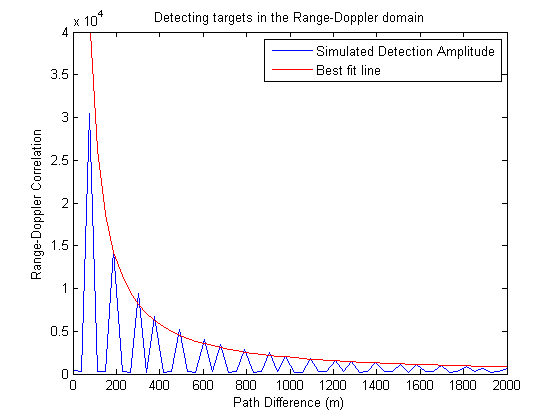
\includegraphics{detect.png}
\caption{Target detection characteristics in the Range-Doppler domain}
\label{fig:detect}
\end{figure}

\begin{figure}[p]
\centering
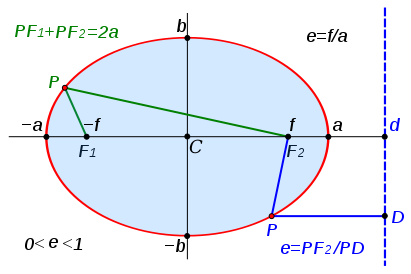
\includegraphics{ell1.png}
\caption{Ellipse and some mathematical properties \cite{ellPic}}
\label{fig:ell1}
\end{figure}

\cleardoublepage

\chapter{Results and Conclusions}

\section{Results}
\label{sec:res}
The Range-Doppler Transformation algorithm described in the previous section was then implemented and tested. The base test case involved a receiver array of 16 radar receiver in a 4 by 4 array. These receivers were centred at the origin and spaced a distance of 200 m away from the next closest receiver. A single transmitter was positions at the co-ordinates $(x,y) = (1000,0)$. 

\bigskip

This scenario was then tested with multiple permutations of zero to four targets. These targets were selected so that they sometimes overlapped in the frequency domain, sometimes overlapped in the range domain, and sometimes overlapped in both. The algorithm was able to handle all of these cases.

\bigskip

One of the reasons that it was able to be so robust to these sorts of shadows, is because of the multiple redundancies in the receivers. A target that may be shadowed by another target in the Range-Doppler map of one receiver, may have them spatially, or frequency separated in the map of another receiver. It is this robustness to both target shadows and ambiguity functions that makes this algorithm so effective.

\bigskip

One such scenario that illustrates this point well is this example case with two receivers
\begin{itemize}
\item{One target located at $(1100,500)$ with velocity vector of $(200,-200)$,}
\item{The second target being stationary and located at $(0,700)$.}
\end{itemize}

\bigskip

A graph showing the Range-Doppler maps for all of the receivers shows that some of them have two distinct targets in this domain, some have the targets blurred together at the same range, and some others can only detect one of the targets. This graph can be seen in figure~\ref{fig:rdbig}.

\begin{figure}[p]
\centering
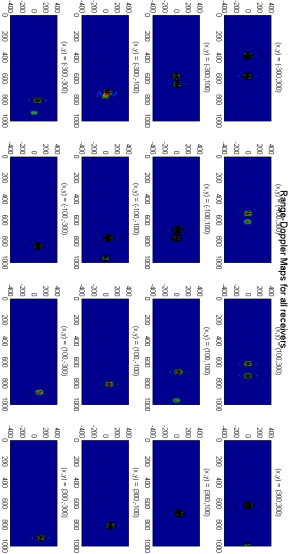
\includegraphics{rdbig2.png}
\caption{Collection of Range-Doppler maps for receiver array with two simulated targets}
\label{fig:rdbig}
\end{figure}

\bigskip

The spatial domain plot showing all of the receivers, transmitters and ellipses due to detected targets in the Range-Doppler maps appears below in figure~\ref{fig:xyell}. This figure clearly shows an abundance of intersection points around the target located at $(1100,500)$. There is also a slightly smaller concentration of intersections at the second target's location $(0,700)$. This position has fewer intersections because of the aforementioned Range-Doppler maps with only one visible target. 

\begin{figure}[p]
\centering
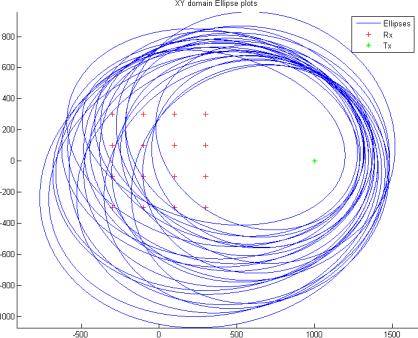
\includegraphics{xyell6.png}
\caption{Spatial domain plot of all receivers, transmitters, and Range-Doppler map transformed ellipses}
\label{fig:xyell}
\end{figure}

\bigskip

The output of the algorithm is just two points, as seen in figure~\ref{fig:rdout}. These points are

\begin{itemize}
	\item{$(1077,520)$ - a distance of 30 m from the actual target at $(1100,500)$}
	\item{$(-45,675)$ - a distance of 51 m from the actual target at $(0,700)$}
\end{itemize}

\begin{figure}[p]
\centering
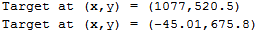
\includegraphics{rdout.png}
\caption{Output of the Range-Doppler Transform Algorithm}
\label{fig:rdout}
\end{figure}

\bigskip

So the algorithm was able to predict, to a high degree of accuracy, the fact that there were targets present, the exact number of targets, and the precise location of the targets. The maximum resolution attainable for a sampling frequency of 8 MHz was calculated to be 37.5 m in section~\ref{sec:TFE}. The fact that this algorithm is getting errors at this order of magnitude tells us that it is extremely accurate for the given sampling frequency.

\bigskip

This algorithm is also robust to timing and synchronisation errors, as the raw data is not sent to the centralised computer. Instead, only the ellipse parameters are sent, which are much more robust to timing errors. A synchronisation error of 1 sample in other algorithms can lead to an error as big as the maximum resolution of 37.5 m. In Range-Doppler transformations, a synchronisation error of 1 sample can only lead to an error of at most the distance that a target can move in that time. A target would need to be travelling at the speed of light\footnote{Because \mbox{$v = \frac{d}{t} = \frac{d}{\frac{1}{f_s}} = d\times f_s = 37.5\times 8e6 = C$}} for the error due to synchronisation to matter for the Range-Doppler transformation.

\newpage
\section{Conclusions}

This thesis has studied the topic of Passive Radar, and proposed a new algorithm for solving the passive radar detection problem. The Range-Doppler Transformation is a novel algorithm intended for use in passive radar detection schemes with large arrays of receivers. It has shown to be successful in medium scale simulations, as well as having a very high degree of accuracy.

\bigskip

The algorithm has been shown to be robust to many effects that plague current passive radar algorithms when they are implemented in the real world. It has a much better tolerance to timing and synchronisation effects, meaning that it is easier to set up a live system.

\bigskip

The multiple redundancies due to the large number of receivers means that even if a target falls within the ambiguity function of another target and cannot be distinguished at one receiver, these two targets are very like to be distinguishable at other receivers. This means that more targets will be able to be detected in more situations than using other methods.

\bigskip

This algorithm also has a much better time complexity than other naively implemented algorithms. This is mostly due to the fact that a lot of the computation is performed in parallel at the receivers themselves. Another bonus this on-board computation brings, is that instead of streaming all of the raw data to a centralised location for processing, only the ellipse parameters of the detected targets needs to be transmitted. This represents a massive decrease in the amount of bandwidth required for implementing this algorithm.

\bigskip

The Range-Doppler transformation algorithm has many strengths both computationally, and with respect to the ease of setting up a real world trial. 

\cleardoublepage

\chapter{Future Directions}

This thesis is complete in the fact that it has achieved all of its goals. However there is always room for further developments and improvements. This section will discuss a few of the directions this project could be taken into the future.

\bigskip

This project could benefit greatly from more analysis of other detection algorithms. Implementing other algorithms similar to this could spawn ideas for new hybrid algorithms, taking the best parts of a number of algorithms. This would require much more time and research into other Passive Radar detection algorithms, and the ability to implement these efficiently.

\bigskip

One of the places where the algorithm can be improved is the detection metric for targets in Range-Doppler domain. Initially, a lot of effort was expended trying to implement a detection system that could be robust and accurate. This method was deemed inappropriate and a global threshold was used instead. This global noise floor threshold could be improved to a better method, that would provide more redundancy and error detection than the current system. 

\bigskip

This algorithm could also be improved to detect the velocity of the target as well. This would involve keeping track of the Doppler shift that correspond to each ellipse, and then calculating the velocity that would cause this Doppler for all of the ellipses that intersect.

\bigskip

Clutter is not considered in this thesis, but if there were to be large numbers of radar receivers, clutter would be an unavoidable problem. A good clutter model could be developed and implemented, perhaps initially by placing random, small RCS targets with zero velocity near the receivers. A method to counteract these effects would need to be developed, perhaps using a Wiener filter, or a Moore-penrose inverse to undo the noise of the clutter.

\bigskip

The Range-Doppler transformation algorithm would greatly benefit from being implemented in a language that is better suited for the voting and consensus algorithms. Implementing this algorithm in an Object-Oriented environment such a Java or C++ would not only increase the ease of implementation of the voting algorithm, but also probably increase the efficiency of the algorithm.

\bigskip

The voting algorithm itself could also be developed further. Currently the algorithm uses a greedy search for the targets, however better voting algorithms exist, as do ones that run in linear time. Perhaps a non-greedy algorithm would deliver better results, or a more tried and tested algorithm, like the RANSAC algorithm could be implemented for this case. Either way, more analysis of the voting and consensus step is definitely required.

\bigskip

The tests that the algorithm passed were mostly small scale tests in the context of the motivation of the algorithm design. More testing would need to be done to confirm the accuracy and scalability of this algorithm if it were to be deployed in the real world.

\bigskip

A small scale deployment of receivers could be used to test this algorithm in the real world. Because of the robustness to timing and synchronisation errors, this would be easier to implement than other passive radar detection schemes. 

\bigskip

Finally, more analysis can be done on the Range-Doppler transformation algorithm itslef. A Receiver operator characteristic analysis could be performed to determine how the system responds to different thresholds and allowances. This would be useful in comparing the algorithm's accuracy to other algorithms.


\appendix

% Chapters after the \appendix command are lettered, not numbered.
% Setting apart the appendices in the table of contents is awkward:

\newpage
\addcontentsline{toc}{part}{Appendices}
\mbox{}
\newpage

% The \mbox{} command between two \newpage commands gives a blank page.
% In the contents, the ``Appendices'' heading is shown as being on this
% blank page, which is the page before the first appendix.  This stops the
% first appendix from be listed ABOVE the word ``Appendices'' in the
% table of contents.

% \include appendix chapters here.

\chapter{Program listings}

This appendix will list some of the most important MATLAB files used in this thesis. For a full code listing, see the companion disk.

\section{Generalised Canonical Correlation Analysis}
This section will list some of the code used in making and testing the GCCA method.
\subsection{Signal Generation}
\label{app:siggen1}
This file, \verb+signal_gen.m+, lists the signal generation that was used for testing the GCCA algorithm
\begin{spverbatim}
function [phi, direct] = signal_gen(posRx, posTx, posTarg, freq, N, noise)
%A function that generates random signal, then distributes it as well as
%off 1 target
%
%ALL DISTANCES ARE IN METRES
%
%INPUTS:
%   posRx - the position of each receiver so that posRx(1,i) and posRx(2,i)
%         are the x- and y-positions of receiver i
%   posTx - the position of the transmitter so that posTx = [xpos; ypos]
%   posTarg - the positions of the targets so that
%           posTarg(:,i) = [xpos taget i; ypos target i]
%   freq - The sampling frequency of the sampled signals
%   N - The number of samples we want generated
%   noise - Optional, 
%
%OUTPUTS:
%   phi - An array of inputs from receivers in the form [X1, X2,...,Xm]
%         where Xi is a column array of values. Xi can be recovered by
%         Xi = phi(:,i)
%   direct - A vector of the direct path signal from Tx to Rx1 only

%CONSTANTS
%C = Speed of light (in m/s)
C = 299792458;
%alpha = Signal degredation (/m or m^-1) Range: 0-1;
%0 is full signal degredation and 1 is none
%alpha = 1;

%CHANGES:
%
%posRx(:,1)  = [x1;y1] of the directional receiver

if nargin<5
    error('There must be at least 5 arguements');
elseif nargin==5
    noise = 0;
end

%DERIVED CONSTANTS
%m = number of receivers
m = size(posRx,2);
%numtarg = number of targets
numtarg = size(posTarg,2);
%dt = time between samples (seconds)
dt = 1/freq;
%DTxTarg = Array of distances where D(i) = distance from transmitter to
%targeti
DTxTarg = zeros(numtarg,1);
for targ = 1:numtarg
    DTxTarg(targ) = norm(posTx-posTarg(:,targ));
end

%DTargRx = Array of distances where D(i,j) = distance from Rxi to target j
DTargRx = zeros(m,numtarg);
for rec = 1:m
    for targ = 1:numtarg
        DTargRx(rec,targ) = norm(posTarg(:,targ)-posRx(:,rec));
    end
end
%DTxRx = Array of distances where D(i) = distance from Tx to Rxi
DTxRx = zeros(m,1);
for rec = 1:m
    DTxRx(rec) = norm(posTx-posRx(:,rec));
end

%Calculate maximum travel time of the signal and the equivelant number of
%samples that it would be delaed by
MAX_DIST = max(DTargRx(:)) + max(DTxTarg);
MAX_TIME = MAX_DIST / C;
MAX_SAMP = round(MAX_TIME / dt)+1;

%Number of generated samples
Ngen = N+MAX_SAMP;
S = randn(Ngen,1) + 1i*randn(Ngen,1);

%Initialize phi (will truncate at end)
phi = zeros(Ngen,m);

% Give each receiver the target signal
% The first signal gets only the direct path signal
for rec = 1:m
    for targ = 1:numtarg
        DIST = DTxTarg(targ) + DTargRx(rec,targ);
        TIME = DIST / C;
        SAMP = round(TIME / dt);
        phi(SAMP:end,rec) = phi(SAMP:end,rec) + S(1:Ngen-SAMP+1);
    end
end

%Give each receiver the original signal
% Only the first signal gets direct path
for rec = 1:m
    DIST = DTxRx(rec);
    TIME = DIST / C;
    SAMP = round(TIME / dt);
%     phi(SAMP:end,rec) = phi(SAMP:end,rec)+S(1:Ngen-SAMP+1);
    if rec==1
        direct = zeros(Ngen,1);
        direct(SAMP:end) = S(1:Ngen-SAMP+1);
        direct = direct(Ngen-N+1:end);
    end
end
  
phi = phi(Ngen-N+1:end,:);
\end{spverbatim}

\subsection{Target Detection}
\label{app:gcca}
This file, \verb+target_detect.m+, implements the GCCA algorithm.
\begin{spverbatim}
function out = target_detect(phi, posRx, posTx, freq, xb, yb, tick)
%A function that returns array of log-likelihood for input phi
%
%ALL DISTANCES ARE IN METRES
%
%INPUTS:
%   phi - An array of inputs from receivers in the form [X1, X2,...,Xm]
%         where Xi is a column array of values. Xi can be recovered by
%         Xi = phi(:,i)
%   posRx - the position of each receiver so that posRx(1,i) and posRx(2,i)
%         are the x- and y-positions of receiver i
%   posTx - the position of the transmitter so that posTx = [xpos; ypos]
%   freq - The sampling frequency of the sampled signals
%
%OPTIONAL INPUTS:
%   xb - the x-boundary. xb = [xmin, xmax]. will iterate over this boundary
%   yb - the y-boundary. yb = [ymin, ymax]. will iterate over this boundary
%   tick - the resolution of the iteration in space
%
%OUTPUTS:
%   out - an array of dimensions [diff(yb), diff(xb)] with log likelihood
%       of each position being a target
%function out

%NOTES:
%   - In code all arrays are row/col == i/j == x/y
%   - At the end out is transposed to get in the correct orientation

%Sort out optional inputs defaults
if nargin < 4
    xb = [-5500,11000];
    yb = [-2000,2000];
    tick = 10;
end

%CONSTANTS
%C = Speed of light (in m/s)
C = 299792458;

%DERIVED CONSTANTS
%m = number of receivers
m = size(posRx,2);
%num_samp = number of samples of each signal taken
num_samp = size(phi,1);
%dt = time between samples (seconds)
dt = 1/freq;
%

%The possible xy positions to check
x = xb(1):tick:xb(2);
y = yb(1):tick:yb(2);

out = zeros(numel(x),numel(y));

%Iterate through each xy position and receiver
iindex = 0;
for i = x
    iindex = iindex + 1;
    jindex = 0;
    for j = y
        jindex = jindex+1;
        
        %Iterate through each receiver to get the time delay and calculate
        %the number of samples delay to put in nset - the set of sample delays
        nset = zeros(m,1);        
        for rec = 1:m
            %Calculate distance along Target - Rx and time taken
            %Can ignore distance from Tx to ij as is constant for each
            %receiver and ij.
            distRx = norm(posRx(:,rec)-[i;j]);
            travel_time = distRx/C;
            
            %calculate n, number of samples delayed
            nset(rec) = round(travel_time / dt);
        end
        
        %time adjusted signal x'(t) and put into PHI
        %Need to set maxn        
        %Shortest delay will be our starting point
        n = min(nset);
        nset = nset - n;
        %Longest delay will determine how many signals we store for each
        nmax = max(nset);
        nstore = num_samp - nmax;
        
        %Initialise the PHI from paper. PHI = [X1' X2' ... Xm']
        %Note: here X1' does not denote transpose
        PHI = zeros(nstore,m);   
         
        for rec = 1:m
            %So we can throw away the first nset samples of each signal to
            %get all signal from the same time
            nstart = nset(rec)+1;
            PHI(:,rec) = phi(nstart:nstart+nstore-1,rec);
        end
        %Here we have PHI for the position (i,j)
        %Calculate Gram Matrix G:
        G = PHI' * PHI;
        out(iindex,jindex) = max(eig(G));
    end
end            
out = out';
out = flipud(out);
\end{spverbatim}

\subsection{Extract Targets}
\label{IP}
This file, \verb+IP_targets.m+, determines the location of the targets from the PPI map generated in \verb+target_detect.m+.

\begin{spverbatim}
function out = IP_targets(im)
im=imdilate(im,strel('disk',2,0));
M = round(size(im,1)/2);
N = round(size(im,2)/2);
mask = zeros(size(im));
for i=1:size(mask,1)
    for j=1:size(mask,2)
        if abs(i-M)+abs(j-N)<50
            mask(i,j) = 1;
        end
    end
end

im=im2bw(im,0.8) & not(mask);

CC = bwconncomp(im);

if CC.NumObjects == 0
    out = [];
else
    out = zeros(2,CC.NumObjects);
    for i=1:CC.NumObjects
        [x,y] = ind2sub(size(im),CC.PixelIdxList{i});
        out(:,i) = [mean(x);mean(y)];
    end
end
\end{spverbatim}

\subsection{Analysis}
This file, \verb+test_canon.m+, sets up a scenario to run and test the GCCA algorithm. It also performs analsis on the results and displays a graph of the findings.
\begin{spverbatim}
%test_canon.m
%Test Generalised canonical correllation
%There will initially be 5 receivers spaced 50m apart located at origin
%(0,0), (0,50), (0,-50), (-50,0), (50,0)
posRx = [0, 0, 0, -50, 50;
         0,50,-50, 0,  0];   
% posRx = [0,0,0;0,50,-50];

%The transmitter will be located 1km East of the receivers
posTx = [1000;0];

%There will be two stationary targets located [[x;y]   [x;y]   [x;y] ...]
posTarg = [100, 20;
          -150, 100];

%Area to check over
xb = [-200,200];
yb = [-200,200];
tick = 1; %increments

%Sampling Frequency of 220MHz
freq = 220e6;

%Will start with 1000 samples
N = 1000;

%Generate the signals
phi = signal_gen(posRx,posTx,posTarg,freq,N);
%%
%SOLVE THE SYSTEM
tic;
out = target_detect2(phi, posRx, posTx, freq, xb, yb, tick);
timeTaken = toc;
disp(['Time taken is ' num2str(timeTaken) ' seconds']);
%%
%Plot it all
% imshow(mat2gray(out));
% colormap(jet);
% out2 = out/max(out(:));
out2 = mat2gray(out);
figure;
imshow(out2);
colormap(jet);
caxis([min(min(out2)) 1]);
hold on;
h = colorbar;
set(h, 'ylim', [min(min(out2)) 1]);
set(get(h, 'Ylabel'),'String','Normalised Likelihood of target');

%plot the receivers
plot(posRx(1,:)-xb(1)+1,posRx(2,:)-yb(1)+1,'o','MarkerEdgeColor','k',...
    'MarkerFaceColor','m','LineWidth',2,'MarkerSize',10);

targ = IP_targets(out2);
if size(targ,2)>0
    plot(targ(2,:),targ(1,:),'o','MarkerEdgeColor','k',...
    'MarkerFaceColor','n','LineWidth',2,'MarkerSize',10);
end

axis on
%Relabel the axes correctly
tick_spacing=50;
ttk = tick_spacing/tick;
set(gca,'YTick',1:ttk:diff(yb)+1);
% set(gca,'YTickLabel','200|150|100|50|0|-50|-100|-150|-200')
set(gca,'YtickLabel',num2str(-tick*(str2num(get(gca,'YTickLabel'))-1)+yb(2)));

set(gca,'XTick',1:ttk:diff(xb)+1);
%set(gca,'XTickLabel','-200|-150|-100|-50|0|50|100|150|200')
set(gca,'XtickLabel',num2str(tick*(str2num(get(gca,'XTickLabel'))-1)+yb(1)));

%TAKES 21.8 seconds (19.5s)
%35.1 with power_method.m

legend('Receiver Location','Detected Target','location','southwest');
title('Plan Position Indicator for Generalised Canonical Correlation');
xlabel('Distance in x-direction (m)');
ylabel('Distance in y-direction (m)');
\end{spverbatim}

\section{Range-Doppler Transformation}
\label{app:rdt}
This section will list some of the code used in making and testing the Range-Doppler Transformation method.
\subsection{Signal Generation}
The code for signal generation for the RD transformation was made a little cleaner and added some extra functionality compared with the code used for GCCA. Again this file is called \verb+signal_gen.m+.

\begin{spverbatim}
function [phi, generated, sig_noise, rxdirect] = signal_gen(posRx, posTx, Targ, freq, carrier_freq, N, SNR)
%A function that generates random signal, then distributes it as well as
%off 1 target
%
%ALL DISTANCES ARE IN METRES
%
%INPUTS:
%   posRx - the position of each receiver so that posRx(i,1) and posRx(i,2)
%         are the x- and y-positions of receiver i
%   posTx - the position of each transmitter so that posTx(i,1) and
%         posTx(i,2) are the x- and y-positions of transmitter i
%   Targ - the positions and velovities of the targets so that
%           posTarg(i,:) = [xpos, ypos, xvel, yvel] of target i
%   freq - The sampling frequency of the sampled signals
%   carrier_freq - The carrier waves frequency
%   N - The number of samples we want generated
%   SNR - Optional - specify the SNR of the AWGN in dB. Default is 100dB
%
%OUTPUTS:
%   phi - An array of inputs from receivers in the form [X1, X2,...,Xm]
%         where Xi is a column array of values. Xi can be recovered by
%         Xi = phi(:,i)
%   direct - A vector of the direct path signal from Tx to Rx1 only

%%%%%CHECK INPUTS%%%%%
%CONSTANTS
%C = Speed of light (in m/s)
C = 299792458;

%Amplifying factor for the radar equation
GAIN = 1000; %GAIN = sqrt(Gt * Gr * Aeff / (4pi))
%Gain for RCS equation
SIGMA = 10; % SIGMA = sqrt(RCSarea / (4pi))

if nargin<6
    error('There must be at least 6 arguements');
elseif nargin==6
    SNR = 1e2;
end

%DERIVED CONSTANTS
%nrx = number of receivers
nrx = size(posRx,1);
%ntx = number of transmitters
ntx = size(posTx,1);
%ntarg = number of targets
ntarg = size(Targ,1);
%dt = time between samples (seconds)
dt = 1/freq;

%DTxTarg = Array of distances where D(i,j) = distance from Txi to target j
DTxTarg = zeros(ntx,ntarg);
for i = 1:ntx
    for j = 1:ntarg
        DTxTarg(i,j) = norm(posTx(i,:)-Targ(j,1:2));
    end
end

%DRxTarg = Array of distances where D(i,j) = distance from Rxi to target j
DRxTarg = zeros(nrx,ntarg);
for i = 1:nrx
    for j = 1:ntarg
        DRxTarg(i,j) = norm(posRx(i,:)-Targ(j,1:2));
    end
end

%DTxRx = Array of distances where D(i,j) = distance from Txi to Rxj
DTxRx = zeros(ntx,nrx);
for i = 1:ntx
    for j = 1:nrx
        DTxRx(i,j) = norm(posTx(i,:)-posRx(j,:));
    end
end

%Frequency shift matricies
%FShift(tx,rx,targ) = frequency shift of signal from tx to targ to rx
FShift = zeros(ntx,nrx,ntarg);
for tx = 1:ntx
    for rx = 1:nrx
        for targ = 1:ntarg
            a = Targ(targ,3:4); %Velocity of target (Vx,Vy)
            b = Targ(targ,1:2) - posTx(tx,:);
            c = Targ(targ,1:2) - posRx(rx,:);
            rtx = dot(a,b) / norm(b);   %Component of Tx/Targ motion
            rrx = dot(a,c) / norm(c);   %Component of Rx/Targ motion
            FShift(tx,rx,targ) = rtx + rrx;
        end
    end
end
%%%ACCOUNT FOR FREQ SAMPLING SHIFT
FShift = FShift * carrier_freq / C; %Correct for actual shift

%Calculate maximum travel time of the signal and the equivelant number of
%samples that it would be delayed by
%Not actual maximum, but an upper bound
MAX_DIST = max([DRxTarg(:);0]) + max([DTxTarg(:);0]);
%Case when no targets:
MAX_DIST = max([DTxRx(:);MAX_DIST]);

MAX_TIME = MAX_DIST / C;
MAX_SAMP = round(MAX_TIME / dt)+1;

%Number of generated samples
Ngen = N+MAX_SAMP;
S = randn(Ngen,1) + 1i*randn(Ngen,1);

%Time vector for frequency shifting
timevec = 0:dt:dt*(Ngen-1);
timevec = timevec'; %ensure column

%Initialize phi (will truncate at end)
phi = zeros(Ngen,nrx);

% Give each receiver the signal from each target and transmitter
for trans = 1:ntx
    for rec = 1:nrx
        for targ = 1:ntarg
            R1 = DTxTarg(trans,targ);
            R2 = DRxTarg(rec,targ);
            DIST = R1 + R2;
            TIME = DIST / C;
            SAMP = round(TIME / dt);
            %Get the signal and frequency correct it
            sig = S.*exp(1i*2*pi*FShift(trans,rec,targ)*timevec);
            %Get the correct part of the signal (wrt time)
            sig = sig(1:Ngen-SAMP+1); 
            AMP = GAIN*SIGMA / (R1*R2); %Signal amplitude
            
            phi(SAMP:end,rec) = phi(SAMP:end,rec) + AMP*sig;
        end
    end
end

%Direct path signal
rxdirect = zeros(size(phi));
%Give each receiver the direct path signal
for rec = 1:nrx
    for trans = 1:ntx
        DIST = DTxRx(rec);
        TIME = DIST / C;
        SAMP = round(TIME / dt); %Number of samples delayed by
        AMP = (GAIN / DIST); %Signal amplitude scaling factor
        phi(SAMP:end,rec) = phi(SAMP:end,rec)+AMP*S(1:Ngen-SAMP+1);
        rxdirect(SAMP:end,rec) = rxdirect(SAMP:end,rec) + AMP*S(1:Ngen-SAMP+1);
    end
end

%Get only the relevant signals
phi = phi(Ngen-N+1:end,:);
rxdirect = rxdirect(Ngen-N+1:end,:);

%Generate noise and add noise
noise = rms(phi(:,1))*10^(-SNR/10);
sig_noise = noise*(randn(size(phi)) + 1i*randn(size(phi)));
phi = phi + sig_noise;
%Add noise to direct path signal as well
noise = rms(rxdirect(:,1))*10^(-SNR/10);
sig_noise = noise*(randn(size(phi)) + 1i*randn(size(phi)));
rxdirect = rxdirect + sig_noise;

generated = S;
\end{spverbatim}

\subsection{Range Doppler Map}
This file, \verb+rangedopplerfft.m+, calculates the Range-Doppler map from a given receiver. It uses the fast Fourier transform.

\begin{spverbatim}
%Generates the range doppler map for a given receiver over a specified
%range of inputs

function [rdmap, ranges, freqs] = rangedopplerfft(phi, freq, range, freqs, rxdirect)
%Inputs
%   phi is an Nx1 column vector of the samples received at receiver of
%   interest.
%   freq is the sampling freq in Hz
%   range is the maximum range of interest in metres. range>0
%   freqs is similar to ranges except for frequencies of interest. freqs is
%   in Hz

%Implemented using FFT's:
%Rxy(t) = x(t) (conv) y*(-t)
%fft(Rxy) = X(f) Y*(f)
%Rxy(t) = ifft( X(f)Y*(f) )

%CONSTANTS
%C = Speed of light (in m/s)
C = 299792458;

%The period (ie time for 1 sample)
dt = 1/freq;

%Work out the maximum ranges
travel_time = range/C;
n = ceil(travel_time/dt); %The number of shifts we need to do
N = n + size(phi,1); %Size to pad to for fft

%Work out the non direct (ie target path) signal
tar = phi - rxdirect;

%Pad out the inputs so we don't get overlap in frequency domain
Fdirect = conj(fft(rxdirect,N)); %Fourier transform of direct path signal

%The range doppler map
rdmap = zeros(n,numel(freqs));

%Time vector for frequency shifting
t = 0:dt:dt*(numel(phi)-1);
t = t';

%We will be taking conjugates in frequency domain, so
freqs = -freqs;

j=0; %index
for f = freqs
    j=j+1; %index
    
    %frequency correct the signal
    fc_sig = tar.*exp(-1i*2*pi*f*t);
    
    %Compute conjugate of FFT
    Fsig = fft(fc_sig,N);
    
    %Find the correlation for all ranges
    cor = ifft(Fdirect.*Fsig);
    
    rdmap(:,j) = cor(1:n);
end

%Get real values
rdmap = abs(rdmap);
% rdmap = abs(rdmap) + real(rdmap);

%return the ranges
ranges = linspace(0,range,n);
\end{spverbatim}


\subsection{Generate Receiver Array}
This file, \verb+getMultRXPos.m+, generates all of the receiver positions in an array.
\begin{spverbatim}
function posRx = getMultRXPos(nx, ny, Rdist)
%Takes a number of points in the x- and y- directions and a distance
%between them and returns an (nx*ny)-by-2 array containing all of the
%locations of the receivers

XS = (nx-1)*Rdist;
YS = (ny-1)*Rdist;
XV = linspace(-XS/2, XS/2, nx);
YV = linspace(-YS/2, YS/2, ny)';
XA = repmat(XV,ny,1);
YA = repmat(YV,1,nx);

posRx = [XA(:), YA(:)];
\end{spverbatim}

\subsection{Target Detection}
\label{app:tdetect}
This file, \verb+detectTarg+, detects the locations of targets in the area from the range-doppler map.

\begin{spverbatim}
function [rdHits, rdMapDetect] = detectTarg(rdmap, ranges,freqs, SNR, PSNR)
%Detects the locations of targets in the area from the range-doppler map
%using the coefficients of P, that are calculated in the function
%detectModel.
%
%rpmap is a range doppler map
%ranges are the set of ranges that the rdmap takes up
%   size(rdmap,1)==size(ranges,2)
%P = [snrs, level] where snrs is an mx1 matrix with possible SNR values and
%level is and m-by-1 matrix with the corresponding noise floor.
%SNR is the SNR level where the map was recorded
%
%rdHits is the resulting target in the for [Range, Doppler]
%rdMapDetect is the same size as rdmap that is passed into the function but
%with 1's where the targets are and 0's elsewhere

if nargin < 5
    load('PSNR.mat')
end

scale = 20; %The error factor in the model

%We first truncate all non interesting information
%find the noise floor
snrs = PSNR(:,1);
[~,idx] = min(abs(snrs-SNR));
cutOff = scale * PSNR(idx,2);

trunc = rdmap > cutOff;

%Do some Image processing techniques to get hits
s  = regionprops(trunc', 'centroid');
cent = round(cat(1, s.Centroid));
rdMapDetect = zeros(size(rdmap));
for i=1:size(cent,1)
    rdMapDetect(cent(i,1),cent(i,2)) = 1;
end

%Now do the processing for the maximum points
[m, id] = max(rdmap,[],2);
ids = m > cutOff;
ID = id(ids);

%Care for the case where there are no targets
if numel(cent)==0
    rdHits = [];
else
    rdHits = [ranges(ids)', freqs(ID)'];
end

% figure;
% subplot(1,2,1); imagesc(rdmap');
% subplot(1,2,2); imagesc(cutOff'); pause;
\end{spverbatim}

\subsection{Determine Ellipse Parameters}
\label{app:ellParam}
This function, \verb+getEllParam.m+, returns the parameters for an ellipse with given constraints.

\begin{spverbatim}
function param = getEllParam(posRx, posTx, pd)
%Gets the ellipse parameters in a common form from
%   Receiver position (posRx)
%   Transmitter position (posTx)
%   path difference as calculated in the range doppler map (pd)
%
%param = [qxx, qyy, qxy, qx, qy, q0] where the ellipse ifs given by:
%
% qxx*x^2 + qyy*y^2 + qxy*x*y + qx*x + qy*y + q0 = 0;

%Extract the positions
x0 = posRx(1); y0 = posRx(2);
x1 = posTx(1); y1 = posTx(2);

%Find middle of ellipse
xm = (x0+x1)/2;
ym = (y0+y1)/2;

DTxRx = norm(posRx - posTx);

%Find angle alpha
alpha = atan((y1-y0)/(x1-x0));

%Find semimajor radii
A = (DTxRx + pd)/2;
f = DTxRx/2;
B = sqrt(A^2-f^2);

ca = cos(alpha);
sa = sin(alpha);
%Get the product terms
qxx = (ca/A)^2 + (sa/B)^2;
qyy = (sa/A)^2 + (ca/B)^2;
qxy = 2*ca*sa/A^2 + -2*ca*sa/B^2;
qx = (-2*xm*ca^2 - 2*ym*ca*sa)/A^2 + (-2*xm*sa^2 + 2*ym*ca*sa)/B^2;
qy = (-2*ym*sa^2 - 2*xm*ca*sa)/A^2 + (-2*ym*ca^2 + 2*xm*ca*sa)/B^2;
q0 = (xm^2*ca^2 + 2*xm*ym*ca*sa + ym^2*sa^2)/A^2 + (xm^2*sa^2 - 2*xm*ym*ca*sa + ym^2*ca^2)/B^2 - 1; 
    
param = [qxx, qyy, qxy, qx, qy, q0];
\end{spverbatim}

\subsection{Ellipse Intersections}
\label{app:ellInt}
This file, \verb+findEllIntersect.m+, finds the intersection of two ellipses.

\begin{spverbatim}
function out = findEllIntersect(Qparam, Rparam)
%Finds the intersection of 2 ellipses given their parameters:
%param = [qxx, qyy, qxy, qx, qy, q0] where the ellipse ifs given by
%qxx*x^2 + qyy*y^2 + qxy*x*y + qx*x + qy*y + q0 = 0;
%
%out = a n-by-2 array where n is the number of intersections
%   0<=n<=4
%   first col is x coord, second col is y coord

%Get q components
qxx = Qparam(1);
qyy = Qparam(2);
qxy = Qparam(3);
qx = Qparam(4);
qy = Qparam(5);
q0 = Qparam(6);
%Get r components
rxx = Rparam(1);
ryy = Rparam(2);
rxy = Rparam(3);
rx = Rparam(4);
ry = Rparam(5);
r0 = Rparam(6);

z4 = (- qxx^2*ryy^2 + qxx*qxy*rxy*ryy + 2*qxx*qyy*rxx*ryy - qxx*qyy*rxy^2 - qxy^2*rxx*ryy + qxy*qyy*rxx*rxy - qyy^2*rxx^2);
z3 = (qx*qxx*rxy*ryy - 2*qy*qyy*rxx^2 - qxy^2*rxx*ry - 2*qxx^2*ry*ryy - qxx*qy*rxy^2 - 2*qx*qxy*rxx*ryy + qx*qyy*rxx*rxy + qxx*qxy*rx*ryy +
 qxx*qxy*rxy*ry - 2*qxx*qyy*rx*rxy + qxy*qy*rxx*rxy + qxy*qyy*rx*rxx + 2*qxx*qy*rxx*ryy + 2*qxx*qyy*rxx*ry);
z2 = (q0*qxy*rxx*rxy - qy^2*rxx^2 - q0*qxx*rxy^2 - 2*q0*qyy*rxx^2 -
qxx*qyy*rx^2 - qxy^2*r0*rxx - 2*qxx^2*r0*ryy - qx^2*rxx*ryy -
qxx^2*ry^2 + qxx*qxy*r0*rxy + 2*q0*qxx*rxx*ryy + 2*qxx*qyy*r0*rxx +
qx*qxx*rx*ryy + qx*qxx*rxy*ry - 2*qx*qxy*rxx*ry + qx*qy*rxx*rxy +
qx*qyy*rx*rxx + qxx*qxy*rx*ry - 2*qxx*qy*rx*rxy + qxy*qy*rx*rxx +
2*qxx*qy*rxx*ry);
z1 = (q0*qx*rxx*rxy - qxx*qy*rx^2 - 2*qxx^2*r0*ry - qx^2*rxx*ry -
2*q0*qy*rxx^2 - 2*q0*qxx*rx*rxy + q0*qxy*rx*rxx + qx*qxx*r0*rxy -
2*qx*qxy*r0*rxx + qxx*qxy*r0*rx + 2*q0*qxx*rxx*ry + 2*qxx*qy*r0*rxx +
qx*qxx*rx*ry + qx*qy*rx*rxx);
z0 = - q0^2*rxx^2 + q0*qx*rx*rxx + 2*q0*qxx*r0*rxx - q0*qxx*rx^2 -
qx^2*r0*rxx + qx*qxx*r0*rx - qxx^2*r0^2;

Ys = roots([z4 z3 z2 z1 z0]);

NY = numel(Ys);

sols = [];
for i=1:numel(Ys)
    y = Ys(i);
    w0 = q0 + qy*y + qyy*y^2;
    w1 = qxy*y + qx;
    w2 = qxx;
    Xs = roots([w2 w1 w0]);
    sols = [sols; [Xs, [y;y]]];
end

%Check which are valid solutions
Q = @(x,y) (q0+qy*y+qyy*y^2) + (qxy*y + qx)*x + (qxx)*x^2;
R = @(x,y) (r0+ry*y+ryy*y^2) + (rxy*y + rx)*x + (rxx)*x^2;

out = [];

tol = 1e-6;

for i=1:size(sols,1)
    qval = abs(Q(sols(i,1),sols(i,2)));
    rval = abs(R(sols(i,1),sols(i,2)));
    im1 = abs(imag(sols(i,1)));
    im2 = abs(imag(sols(i,2)));
    if (qval<tol && rval<tol) && (im1<tol && im2<tol)
        out = [out; sols(i,:)];
    end
end

%Find unique up to 5 digits
n = 10^5;
rounded = real(floor(out*n)/n);
[~,ids,~] = unique(rounded,'rows');

out = real(out(ids,:));
\end{spverbatim}

\subsection{Vote and Consensus}
\label{app:vote}
This file, \verb+getTargetLocation.m+, applies the intersection, voting and consensus algorithm.

\begin{spverbatim}
function target = getTargetLocation(rx)
%A function that determines the likely positions of targets from an array
%of static radar receivers
%
%rx is a struct array with feild ellParam describing the parameters of 
%an ellipse for each hit in the range doppler domain

%Minimum distance between any 2 intersections of ellipses
%Should be a funcion of the sampling rate
%C/Fs = 3e8/8e6 = 37.5m
minDist = 4*37.5; %Add in a bit of leeway

%an array containing [xpos, ypos, numInt]
target = zeros(0,3);

%Number of receivers
N = size(rx,1);

for i = 1:N-1
    iParam = rx(i).ellParam;
    for ie = 1:size(iParam,1)
        Ell1 = iParam(ie,:);
        for j = i+1:N
            jParam = rx(j).ellParam;
            for je = 1:size(jParam,1)
                Ell2 = jParam(je,:);
                %Compare Ell1 and Ell2
                inter = findEllIntersect(Ell1, Ell2);
                for id = 1:size(inter,1)
                    testPos = inter(id,:);
                    currentPos = target(:,1:2);
                    %Find the differene in distance
                    dist = currentPos - repmat(testPos,size(currentPos,1),1);
                    dist = hypot(dist(:,1),dist(:,2));
                    %Compare to minimum
                    isLT = dist<minDist;
                    if any(isLT)
                        %We have a match, so increment
                        idMatch = find(isLT,1);
                        %Also update match to average
                        n = target(idMatch,3);
                        target(idMatch,1:2) = (n*target(idMatch,1:2) + testPos) / (n+1);
                        target(idMatch,3) = n+1;
                    else
                        %No match so add position
                        target = [target; [testPos,1]];
                    end
                end 
            end
        end
    end
end

target = sortrows(target,3);
target = target(end:-1:1,:);

if norm(target(1,1:2)-target(2,1:2)) < 500
    %Weighted average the first 2
    n1 = target(1,3);
    n2 = target(2,3);
    tl = (n1*target(1,1:2) + n2*target(2,1:2))/(n1+n2);
    disp(['Target at (x,y) = (' num2str(tl(1),4) ',' num2str(tl(2),4) ')']);
else
    %Weighted average the first 2
    n1 = target(1,3);
    n2 = target(3,3);
    tl = (n1*target(1,1:2) + n2*target(3,1:2))/(n1+n2);    
    disp(['Target at (x,y) = (' num2str(tl(1),4) ',' num2str(tl(2),4) ')']);
    
    m1 = target(2,3);
    m2 = target(4,3);
    t2 = (m1*target(2,1:2) + m2*target(4,1:2))/(m1+m2);    
    disp(['Target at (x,y) = (' num2str(t2(1),4) ',' num2str(t2(2),4) ')']);
end
\end{spverbatim}

\subsection{Test Multiple Receivers}
This file \verb+mult_rx.m+ instantiates a simulation of 1 transmitter, 16 receivers and 2 targets. It also determines the Range-Doppler Map for these and performs the Range-Doppler Transformation algorithm, showing the results graphically.

\begin{spverbatim}
%Test the multiple Rx array

PLOT_RESULTS = true;

%Using 16 receivers in a 4-by-4 array
%Single Transmitter
%Single Target

nx = 4; %number in x-direction
ny = 4; %number in y-direction
Rdist = 200;  %200m apart

posRx = getMultRXPos(nx, ny, Rdist);
posTx = [1000,0];
% Targ = [1100,500,200,-200];
Targ = [1100,500,200,-200;
        0,700,0,0];

freq = 8e6;  %Sampling frequency
cfreq = 220e6; %Carrier frequency
time = 0.01; %seconds
N = time*freq; %Number of samples to generate
SNR = 30; %Higher SNR is better (in dB)

%Detection co-efficients (calculated previously)
load('PSNR.mat');

range = 1000;   %can do 20000 (ie 20km)
freqs = -400:20:400;

%Will store results in a structure array
%Preallocate the array
rx = repmat(struct('loc',0,'rdmap',0,'rdHits',0,'ellParam',[]),nx*ny,1);

if PLOT_RESULTS
    figure;
    suptitle('Range-Doppler Maps for all receivers');
end

tic
for i=1:nx*ny
    [phi, s, noise, rxdirect] = signal_gen(posRx(i,:),posTx,Targ,freq,cfreq,N, SNR);
    [rdmap, ranges] = rangedopplerfft(phi,freq, range, freqs,rxdirect);
    
    %Store the info in the struct array
    rx(i).loc = posRx(i,:);
    rx(i).rdmap = rdmap;
    rx(i).rdHits = detectTarg(rdmap, ranges,freqs, SNR, PSNR);
    
    Nhit = size(rx(i).rdHits,1);
    param = zeros(Nhit,6);
    for j=1:Nhit
        param(j,:) = getEllParam(posRx(i,:),posTx,rx(i).rdHits(j,1));
    end
    rx(i).ellParam = param;
    
    if PLOT_RESULTS
        %Make sure it looks right (plots in the right place)
        [idi, idj] = ind2sub([ny,nx],i);
        idi = mod(-idi,ny)+1;
        sub2ind([nx,ny],idj,idi);
        subplot(ny,nx,sub2ind([nx,ny],idj,idi));
        
        %plot it
        [X,Y] = meshgrid(ranges, freqs);
        contourf(X,Y,rdmap');
        title(['(x,y) = (' num2str(posRx(i,1)) ',' num2str(posRx(i,2)) ')']);
        drawnow;
    end
    
    %Progress bar
    disp(i/nx/ny);
end
TIMER = toc; %time it

disp(['Average time taken to simulate, display and detect is '
num2str(TIMER/nx/ny) ' seconds']);

TARGET_LOC = getTargetLocation(rx);

%Plot the results
[he, hr, ht] = plotAllEll(rx,posTx);
title('XY domain Ellipse plots');
legend([he, hr, ht], 'Ellipses','Rx','Tx');

% Find 1 interection and plot it
ID1 = 13;
ID2 = 16;

intersect = findEllIntersect(rx(ID1).ellParam(1,:),rx(ID2).ellParam(1,:));

figure; hold on;
plotEll(rx(16).ellParam(1,:));
plotEll(rx(13).ellParam(1,:));

for i=1:size(intersect,1)
    plot(intersect(i,1),intersect(i,2),'r*');    
end

plot(rx(16).loc(1),rx(16).loc(2),'g*');
plot(rx(13).loc(1),rx(13).loc(2),'g*');
plot(posTx(1),posTx(2),'m*');
title(['Intersection of 1 point from Rx' num2str(ID1) ' and Rx'
num2str(ID2)]);
\end{spverbatim}

\chapter{Companion disk}

The companion disk contains all of the materials developed during this thesis.
This disk is also available online at \\
https://github.com/lewythefly/ENGG4801-Passive-Radar-Detection

\bigskip

The following information appears in the root directory of the companion CD in the file \verb+readme.txt+.

\begin{spverbatim}
Thesis: Passive Radar Detection using Range-Doppler Transformations
Student: Lewis Chambers
Std #: 42328188
email: lewis.chambers@uqconnect.edu.au
Supervisor: Vaughan Clarkson

This is the base directory for the companion CD.

The completed assessment appears in the folders:
 - A1 Project Proposal
 - A2 Progress Seminar
 - A3 Demonstration
 - A4 Thesis

The endnote data contained in the proposal appears in the folder 'Endnote'.

A backup history is contained in the folder 'History - Backups'.

The files developed for this Thesis are contained in the folder 'MATLAB files'. More detail appears in this folder.

Other refernce material is contained in the folder 'Other'.

Some of the research papers cited in the thesis are contained in the folder 'Research Papers'
\end{spverbatim}
\bigskip
More information is located in the \verb+readme.txt+ file in the folder \verb+MATLAB files+.
\begin{spverbatim}
Note: All folders in this directory with subfolders have a script addp.m. This script will add all of the current directory to the MATLAB path so you can run all of the files.

'Paper 1' contains the working version of GCCA algorithm
'Paper 1 - Optimisation' contains the tested and unsuccessful optimisations using the power method
'Paper 2' contains the incomplete works on Bayesian detection of signals with known rank
'Presentation' contains the files used for the live demo midway through the thesis
'Range Doppler Transform' contains all of the files for the Range Doppler Transform algorithm
'Tests and Exploration' contains some extra files used for testing and understanding of concepts
\end{spverbatim}

\cleardoublepage

\begin{thebibliography}{99}
\addcontentsline{toc}{chapter}{Bibliography}

\bibitem{Willis1} N. J. Willis and H. D. Griffiths, "Advances in bistatic radar (Willis, N.J. and Griffiths, H.D., Eds.; 2007) [Book Review]," \emph{Aerospace and Electronic Systems Magazine, IEEE}, vol. 23, pp. 46-46, 2008.

\bibitem{HK2} H. Kuschel, J. Heckenbach, S. Muller, and R. Appel, "On the potentials of passive, multistatic, low frequency radars to counter stealth and detect low flying targets," in \emph{Radar Conference, 2008. RADAR '08. IEEE}, 2008, pp. 1-6.

\bibitem{Willis} N. J. Willis, \emph{Bistatic radar}. Raleigh, NC: SciTech Publishing, 2005.

\bibitem{Arend} G. W. Arend, "Radar versus Stealth: Passive Radar and the Future of U.S. Military Power," \emph{Joint Force Quarterly : JFQ}, p. 136, 2009

\bibitem{HK5} H. Kuschel, "Approaching 80 years of passive radar," in \emph{Radar (Radar), 2013 International Conference} on, 2013, pp. 213-217.

\bibitem{HK6} H. Kuschel and D. O'Hagan, "Passive radar from history to future," in \emph{Radar Symposium (IRS)}, 2010 11th International, 2010, pp. 1-4.

\bibitem{pic1} GYGES Publishing Company (2014), \emph{The Klein Heidelberg, Luftwaffe radar stations} [online]. Available: http://www.gyges.dk/Klein\%20Heidelberg.htm

\bibitem{LHM} "Lockheed Martin Silent Sentry,"  vol. 150, ed. New York: McGraw Hill Publications Company, 1999, p. 75.

\bibitem{JE8} J. E. Palmer, H. A. Harms, S. J. Searle, and L. Davis, "DVB-T Passive Radar Signal Processing," \emph{IEEE Transactions on Signal Processing}, vol. 61, pp. 2116-2126, 2013.

\bibitem{HD9} H. D. Griffiths and C. J. Baker, "Passive coherent location radar systems. Part 1: performance prediction," \emph{Radar, Sonar and Navigation, IEE Proceedings -}, vol. 152, pp. 153-159, 2005.

\bibitem{gcc} K. S. Bialkowski, I. V. L. Clarkson, and S. D. Howard, "Generalized canonical correlation for passive multistatic radar detection," In \emph{Proc. IEEE Statist. Signal Process. Workshop}, pp. 417-420, 2011.

\bibitem{MB11} M. Bernaschi, A. Di Lallo, A. Farina, R. Fulcoli, E. Gallo, and L. Timmoneri, "Use of a graphics processing unit for passive radar signal and data processing," \emph{Aerospace and Electronic Systems Magazine, IEEE}, vol. 27, pp. 52-59, 2012.

\bibitem{MC12} M. Conti, F. Berizzi, M. Martorella, E. D. Mese, D. Petri, and A. Capria, "High range resolution multichannel DVB-T passive radar," \emph{Aerospace and Electronic Systems Magazine, IEEE}, vol. 27, pp. 37-42, 2012.

\bibitem{MK13} M. Klein and N. Millet, "Multireceiver passive radar tracking," \emph{Aerospace and Electronic Systems Magazine, IEEE}, vol. 27, pp. 26-36, 2012.

\bibitem{GC14} G. C. Carter, "Coherence and time delay estimation," \emph{Proceedings of the IEEE}, vol. 75, pp. 236-255, 1987.

\bibitem{SS15} S. Sirianunpiboon, S. D. Howard, and D. Cochran, "Multiple-channel detection of signals having known rank," 2013, pp. 6536-6540.

\bibitem{DE16} D. E. Hack, L. K. Patton, B. Himed, and M. A. Saville, "On the applicability of source localization techniques to passive multistatic radar," 2012, pp. 848-852.

\bibitem{SFN} Bialkowski, K.S.; Clarkson, I.V.L., "Passive radar signal processing in single frequency networks," \emph{Signals, Systems and Computers (ASILOMAR), 2012 Conference Record of the Forty Sixth Asilomar Conference on} , vol., no., pp.199,202, 4-7 Nov. 2012

\bibitem{CV17} C. V. Verhoosel, M. A. Gutiérrez, and S. J. Hulshoff, "Iterative solution of the random eigenvalue problem," \emph{ed Dordrecht: Springer Netherlands}, 2006, pp. 304-304.

\bibitem{RA18} R. A. Willoughby and J. K. Cullum, \emph{Lanczos algorithms for large symmetric eigenvalue computations} vol. 41. Philadelphia: Society for Industrial and Applied Mathematics, 2002.

\bibitem{IE19} I. Erdelyi, "On speeding convergence of an iterative eigenvalue process," \emph{The Computer Journal}, vol. 8, pp. 159-165, 1965.

\bibitem{AB20} A. Bejan, "Largest eigenvalues and sample covariance matrices. tracy-widom and painleve ii: computational aspects and realization in s-plus with applications," Preprint: \emph{http://www.vitrum.md/andrew/MScWrwck/TWinSplus.pdf}, 2005.

\bibitem{RHB} Merill I Skolnik. Radar Handbook. McGraw-Hill

\bibitem{CMOS} Ning Zhang; Kenneth, K.O., "W-band pulsed radar receiver in low cost CMOS," \emph{Custom Integrated Circuits Conference (CICC), 2010 IEEE} , vol., no., pp.1,4, 19-22 Sept. 2010

\bibitem{lowCost} Flightradar24 (2013) \emph{ADS-B Receiver For Less Than 20 Euros} [online]. Available: http://www.flightradar24.com/dvbt-stick

\bibitem{SNR} M.Skolnik, \emph{Introduction to Radar Systems}, McGraw Hill, 1980

\bibitem{thermal} D.Barton, \emph{Modern Radar Systems Analysis}, Artech, 1988

\bibitem{ellPic} Dave3457 (username), \emph{Ellipse Properties of Directrix and String Construction} [online]. Available: \verb+http://upload.wikimedia.org/wikipedia/commons/6/+
\verb+65/Ellipse_Properties_of_Directrix_and_String_Construction.svg+, 3 Jul. 2010.

\bibitem{proj} Richter-Gebert, J. 2011, \emph{Perspectives on projective geometry: a guided tour through real and complex geometry}, Springer, New York; Heidelberg; Berlin.

\bibitem{intell2} R.G. Edwards, \emph{Solution coordinates for a pair of bivariate quadratic equations}, The Maptoops Company, [online]. Available: \verb+http://www.maptools.home.comcast.net/~maptools/BivariateQuadratics.pdf+, 17 Sep. 2013.

\bibitem{intell3} D. Eberly, \emph{The Area of Intersecting Ellipses}, Geometric Tools, LLC, [online]. Available: \verb+http://www.geometrictools.com/Documentation/AreaIntersectingEllipses.pdf+, 15 Aug. 2014

\bibitem{vote1} R.S. Boyer. In R.S. Boyer (ed.), \emph{Automated Reasoning: Essays in Honor of Woody Bledsoe, Automated Reasoning Series}, Kluwer Academic Publishers, Dordrecht, The Netherlands, 1991, pp. 105-117.

\bibitem{vote2} Parhami, B. 1994, "Voting algorithms", \emph{IEEE Transactions on Reliability}, vol. 43, no. 4, pp. 617-629.

\bibitem{vote3} Kumar, A., "Performance analysis of a hierarchical quorum consensus algorithm for replicated objects," \emph{Distributed Computing Systems, 1990. Proceedings., 10th International Conference on} , vol., no., pp.378,385, 28 May-1 Jun 1990

\end{thebibliography}

\end{document}
